\chapter{研究方法}
\fontsize{12pt}{18pt}\selectfont

% ------------------------- 3.0 ------------------------- %
% 研究目的;研究假設;研究方法
本研究旨在透過探討減少相機使用數量對於人體姿態估計精準度的影響,以提高人體姿態估計的應用性,並探討 IMU 資訊融合在人體姿態估計中的必要性。本研究假設透過減少相機數量,並融合 IMU 資訊,可以有效提高人體姿態估計的成功率,並達成不需 Vicon 資訊,在任何環境下皆可進行人體姿態量測及重建的目標。為了驗證此假設,本研究將進行一系列實驗,並探討減少相機使用數量對於人體姿態估計精準度的影響,以及 IMU 資訊融合在人體姿態估計中的必要性。
研究方法主要分為三大主軸,
介紹如下:
\begin{itemize}
    \item \textbf{主軸一:探討減少相機使用數量對於人體姿態估計精準度的影響}
    \\ 透過學者們提供的 TotalCapture Dataset 進行實驗,探討減少相機使用數量對於人體姿態估計精準度的影響。
    \item \textbf{主軸二:更改三維人體模型建立方法}
    \\ 透過更改三維人體模型的建立方法,探討僅藉由影像辨識工具建立個人化三維人體模型的可行性,藉此達成不借助 Vicon 系統,將 IMU 資料的朝向資訊轉換為位置資訊,進而進行感測器融合。
    \item \textbf{主軸三:資料前處理及感測器融合}
    \\ 透過相機校正、時間同步及空間校正等方法,將影像資料及 IMU 資料進行前處理,並進行感測器融合,輸出三維人體姿態估計結果,證實融合 IMU 資訊可以有效提高人體姿態重建的成功率。
\end{itemize}

% 研究流程圖 + 說明

\clearpage

% ------------------------- 3.1 ------------------------- %
\section{探討減少相機使用數量對於人體姿態估計精準度的影響}
% 探討減少相機使用數量對於人體姿態估計精準度的影響及其擺放位置介紹,可是擺放位置的結論還沒有可以很好的呈現方式,所以暫時先不要有這方面的結論和討論
現階段人體姿態估計的方法多為使用至少四台相機進行影像辨識,並融合 IMU 資訊進行姿態估計,
例如在文獻~\cite{Zhang_2020_CVPR}中,作者使用到 4 台相機及 8 個 IMU 的資料。儘管相機為相對較易取得的感測器,
但是要架設至少 4 台相機並不容易,且相機數量的增加也意味著設備的成本增加,並增加實驗架設的複雜度、降低設備的機動性。
% 另外在 TotalCapture Dataset 發表的文獻~\cite{Trumble:BMVC:2017}中則有提及嘗試減少相機的硬體數量,準確度隨著相機數量的減少而下降,
因此本章節嘗試減少相機數量
% \sout{並選擇相機擺放位置}
進行感測器融合計算,
探討減少相機使用數量對於人體姿態估計精準度的影響
% ,\sout{並嘗試探討相機擺放位置的選擇}
。

\subsection{實驗方法}
% 實驗方法介紹
% 目前的相機用量及擺放位置敘述,要 cite totalcapture 和 data fusion
TotalCapture Dataset~\cite{Trumble:BMVC:2017} 共蒐集了五位受試者的動作資料,每位受試者進行四組動作,每組動作重複三次,每組動作皆提供 8 台相機資料,可將整個實驗場域完整拍攝、13 個 IMU 資料、Vicon 資料,且這些資料已進行時間同步、空間校正,可直接進行感測器融合實驗,因此本研究選擇使用 TotalCapture Dataset 進行實驗。

TotalCapture Dataset 實驗環境為一個 4x6 (m) 的方形空間,每一面牆面上方架設兩台相機,如圖~\ref{ch3_fig_cameraset_totalcap} 所示,四面牆共計八台相機,每台相機距離地面高度皆為 2.5 (m),擺放位置以上視的視角呈現。

\begin{figure}[!ht]
   \centering
   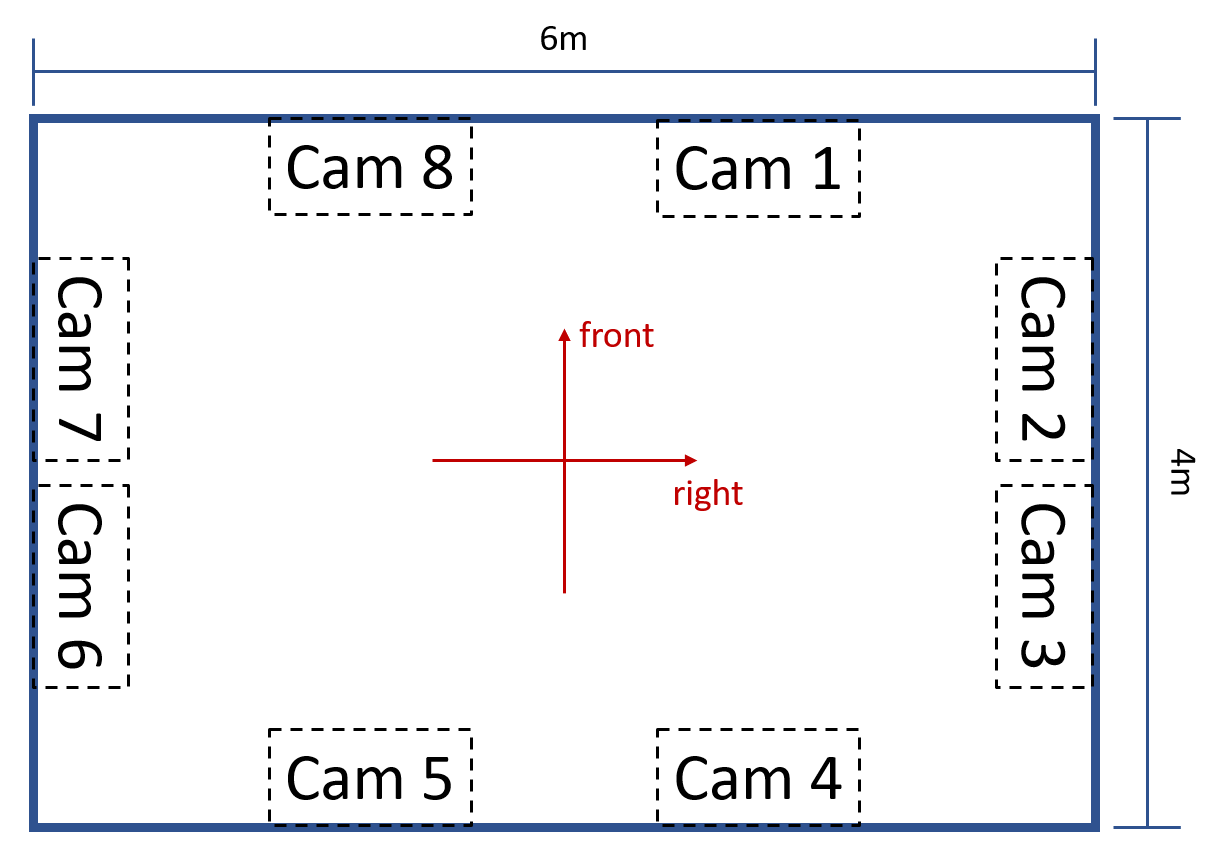
\includegraphics[width=8cm]{figure/ch3_fig_cameraset_totalcap.png}
    \caption[相機擺放位置]{相機擺放位置}
    \label{ch3_fig_cameraset_totalcap}
\end{figure}

本次實驗將分成七類情況進行,每一類情況的實驗流程皆如圖~\ref{ch3_fig_cameraset_flow},首先選擇 x 台相機作為此次實驗資料,並與 IMU 進行感測器融合,接著將估計結果與 Vicon 資訊比對,計算平均每關節誤差 (mean per joint position error, MPJPE),最後計算每一類結果的平均及標準差。

其中,平均每關節誤差 (mean per joint position error, MPJPE) 為常用於評估三維人體姿態估計的指標,計算方式如式~\ref{ch3_equ_MPJPE} ,其中, $N$ 為關節點數量,$p_i$、$q_i$ 分別為關節點的估計座標與真實座標,其概念為取每個關節點估計結果與真實結果間的歐式距離,再將所有關節點的距離值加總後取平均,即為 MPJPE。

\begin{equation}
    MPJPE = \frac{1}{N} \sum_{i=1}^{N} \parallel p_i - q_i \parallel_2
    \label{ch3_equ_MPJPE}
\end{equation}

例如,第一類情況為從八台相機中任選一台相機與 8 個 IMU 進行感測器融合計算,並將得到的姿勢估計結果與 TotalCapture Dataset 提供的 Vicon 位置資料進行比對,計算平均每關節誤差 (mean per joint position error, MPJPE),第二類為任選兩台相機與 8 個 IMU 進行姿勢估計,以此方式遞增至第七類,任選七台相機與 8 個 IMU 進行姿勢估計,每一類情況皆會產生一組 MPJPE 數值,藉由觀察每一類 MPJPE 數值 的平均值及標準差,探討相機的使用數量與姿勢估計的準確度之間的關係。

\begin{figure}[!ht]
   \centering
   
\includegraphics[width=\linewidth]{figure/ch3_fig_cameraset_flow.png}
    \caption[減少相機數量實驗流程]{減少相機數量實驗流程}
    \label{ch3_fig_cameraset_flow}
\end{figure}

% ------------------------- 3.2 ------------------------- %
\section{實驗系統設定與實驗環境}\label{ch3_exp_setting}
% 系統架設;實驗環境
% 說明會講到實驗流程、系統設定、實驗環境等等的事情
進行人體姿勢估計實驗時,需使用多種感測器來量測人體姿態,且需多項事前準備工作及設置,
本章節將會依序說明整體實驗流程、實驗環境、實驗系統設定及實驗動作。

\subsection{實驗方法}
% 講我蒐集資料的事前工作,和整個方法的概述
在進行人體姿態估計的實驗方法如圖~\ref{ch3_fig_exp_flow} 所示,共可分為量測、融合與模擬、驗證重建結果三個階段。於量測階段,首先進行相機內部校正參數 (intrinsic parameters) 及外部校正參數 (extrinsic parameters) 拍攝,拍攝內部參數影片時,需使棋盤格校正板盡可能填滿畫面,並涵蓋多種不同角度的畫面,以便進行內部參數校正,拍攝外部參數影片時,需由受試者站在實驗初始位置並拿著棋盤格校正板,以便進行外部參數校正,與此同時將蒐集校正板上的 IMU 資料,完成相機端的空間校正資料蒐集。
% 接著進行個人化三維人體模型資料蒐集,由受試者站在實驗初始位置,進行時間同步動作後,維持 T-pose 約 1 \textasciitilde\ 2 秒進行拍攝及 IMU 量測,最後再進行一次時間同步動作,完成個人化三維人體模型資料蒐集。
再來即可開始進行實驗動作資料蒐集,由受試者站在實驗初始位置,進行時間同步動作後,進行實驗動作拍攝及 IMU 量測,最後再進行一次時間同步動作,完成實驗動作資料蒐集,以上即為量測階段的資料蒐集工作,接著將蒐集到的影像資料及 IMU 量測資料進行融合及模擬,包括時間同步、空間校正,建立三維人體模型、感測器融合等工作,融合及模擬的輸出即為三維人體姿態估計結果,最後計算肢段長度,並與量測的人體肢段長度比對,進行驗證。

\begin{figure}[!ht]
   \centering
   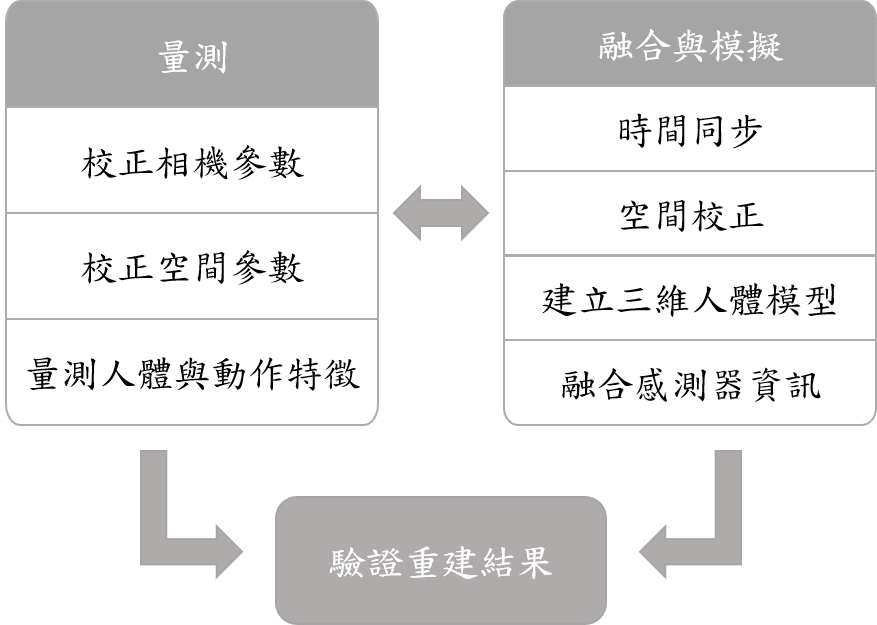
\includegraphics[width=11cm]{figure/ch3_fig_exp_flow.png}
    \caption[人體姿態估計實驗方法]{人體姿態估計實驗方法}
    \label{ch3_fig_exp_flow}
\end{figure}

% \subsection{實驗環境}
% % 實驗環境介紹

\subsection{實驗環境及尺寸}
% 實驗環境介紹
實驗環境空間尺寸為 880$\times$880 (cm),全室拉上遮光布遮蔽室外光線,且實驗背景為單色背景,以減少背景對影像資料的影響。
量測時間為晚上 8 點至 9 點,以確保環境光線穩定,並減少環境光對影像資料的影響。
實驗環境及尺寸如圖~\ref{ch3_fig_indoor_scale} 所示,
受試者初始位置為圖中黑色空心圓圈位置,實驗過程中於 278$\times$283 (cm) 的方形範圍內進行動作,
用於錄製影像的兩台手機位置於圖~\ref{ch3_fig_indoor_scale} 中紅點標示處。
實際實驗環境及受試者位置如圖~\ref{ch3_fig_indoor_position} 所示,圖~\ref{ch3_fig_indoor_position} (a) 為相機與受試者位置的前視情形, cam01 及 cam02 分別於圖中的右側中間位置及圖中的左下位置,圖~\ref{ch3_fig_indoor_position} (b) 為相機與受試者位置的前視情形, cam01 及 cam02 分別於圖中的左側中間位置及圖中的正中位置。

\begin{figure}[!ht]
   \centering
   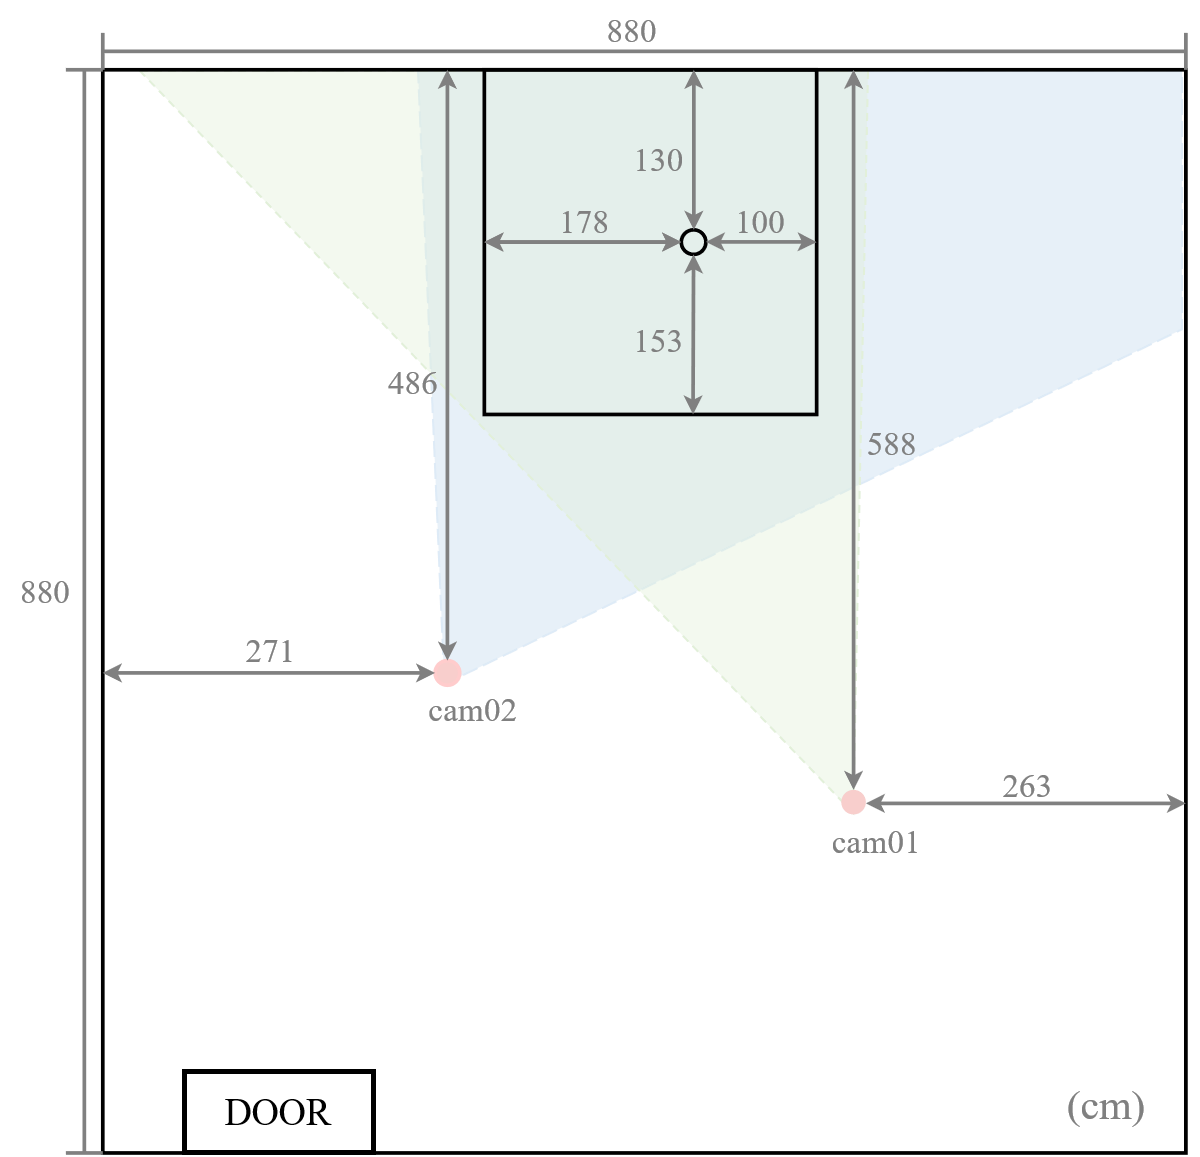
\includegraphics[width=\linewidth]{figure/ch3_fig_indoor_scale.png}
    \caption[實驗環境及尺寸]{實驗環境及尺寸}
    \label{ch3_fig_indoor_scale}
\end{figure}

\begin{figure}[!ht]
   \centering
   \begin{minipage}{.5\textwidth}
     \centering
     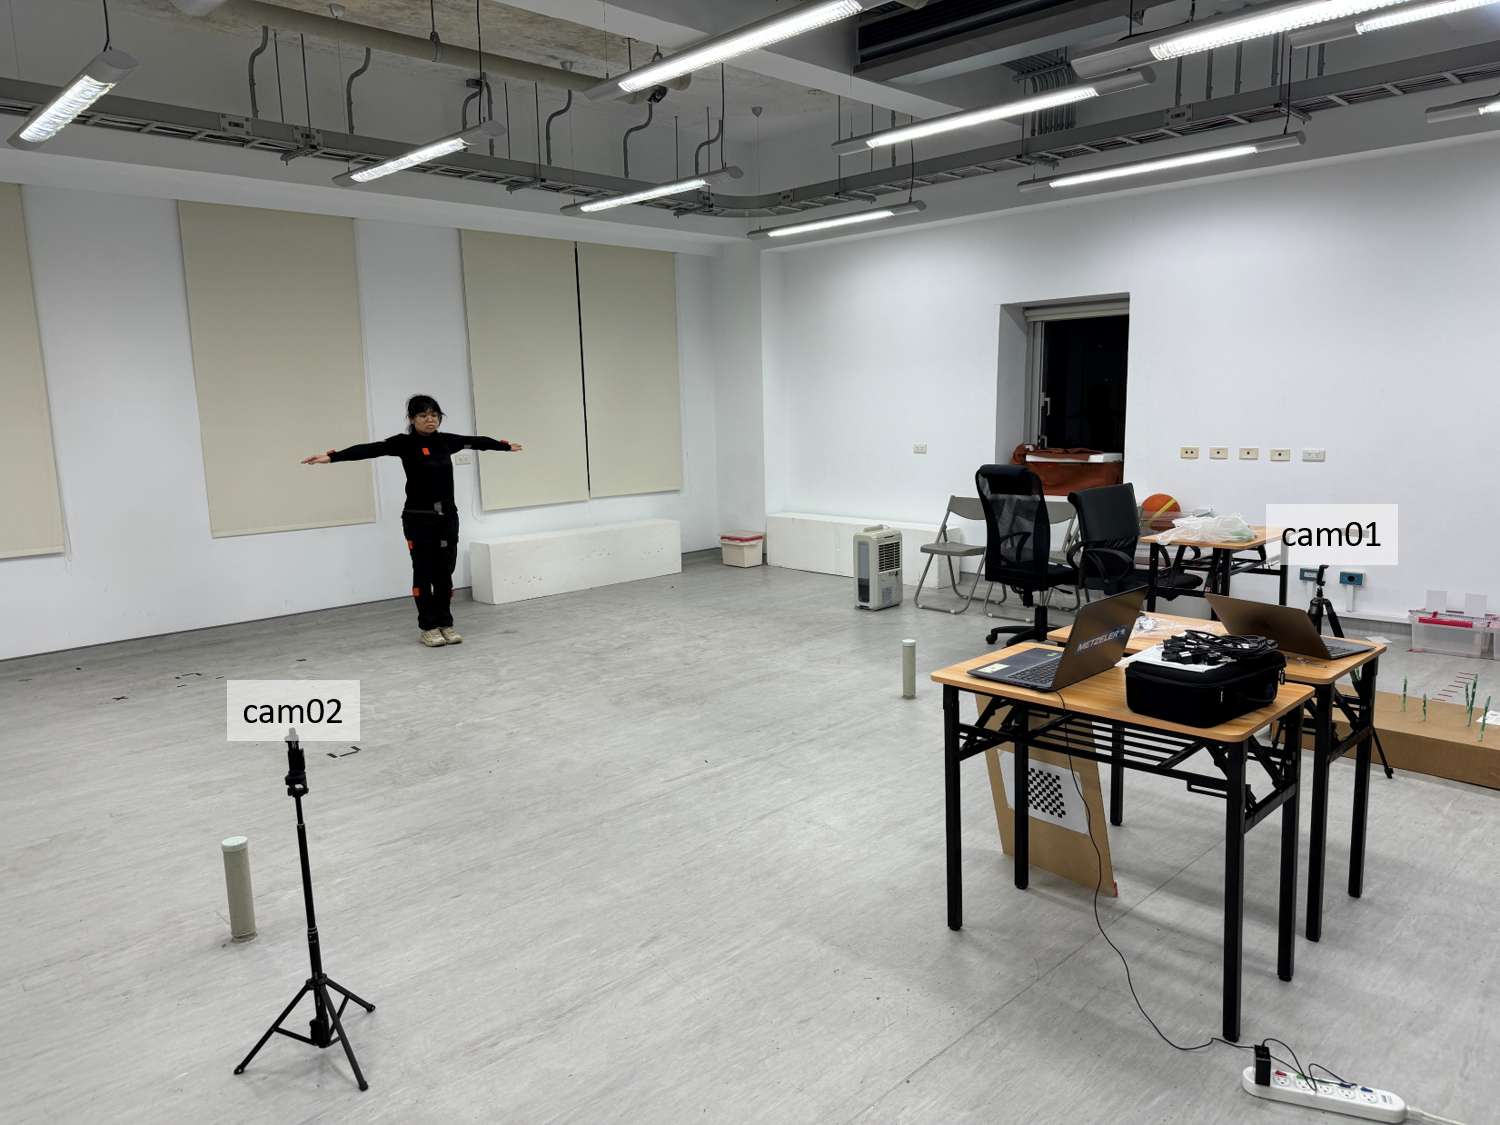
\includegraphics[width=.95\linewidth]{figure/ch3_fig_indoor_position1.png}
     \caption*{(a)相機與受試者位置 (前視)}
   \end{minipage}%
   \begin{minipage}{.5\textwidth}
      \centering
      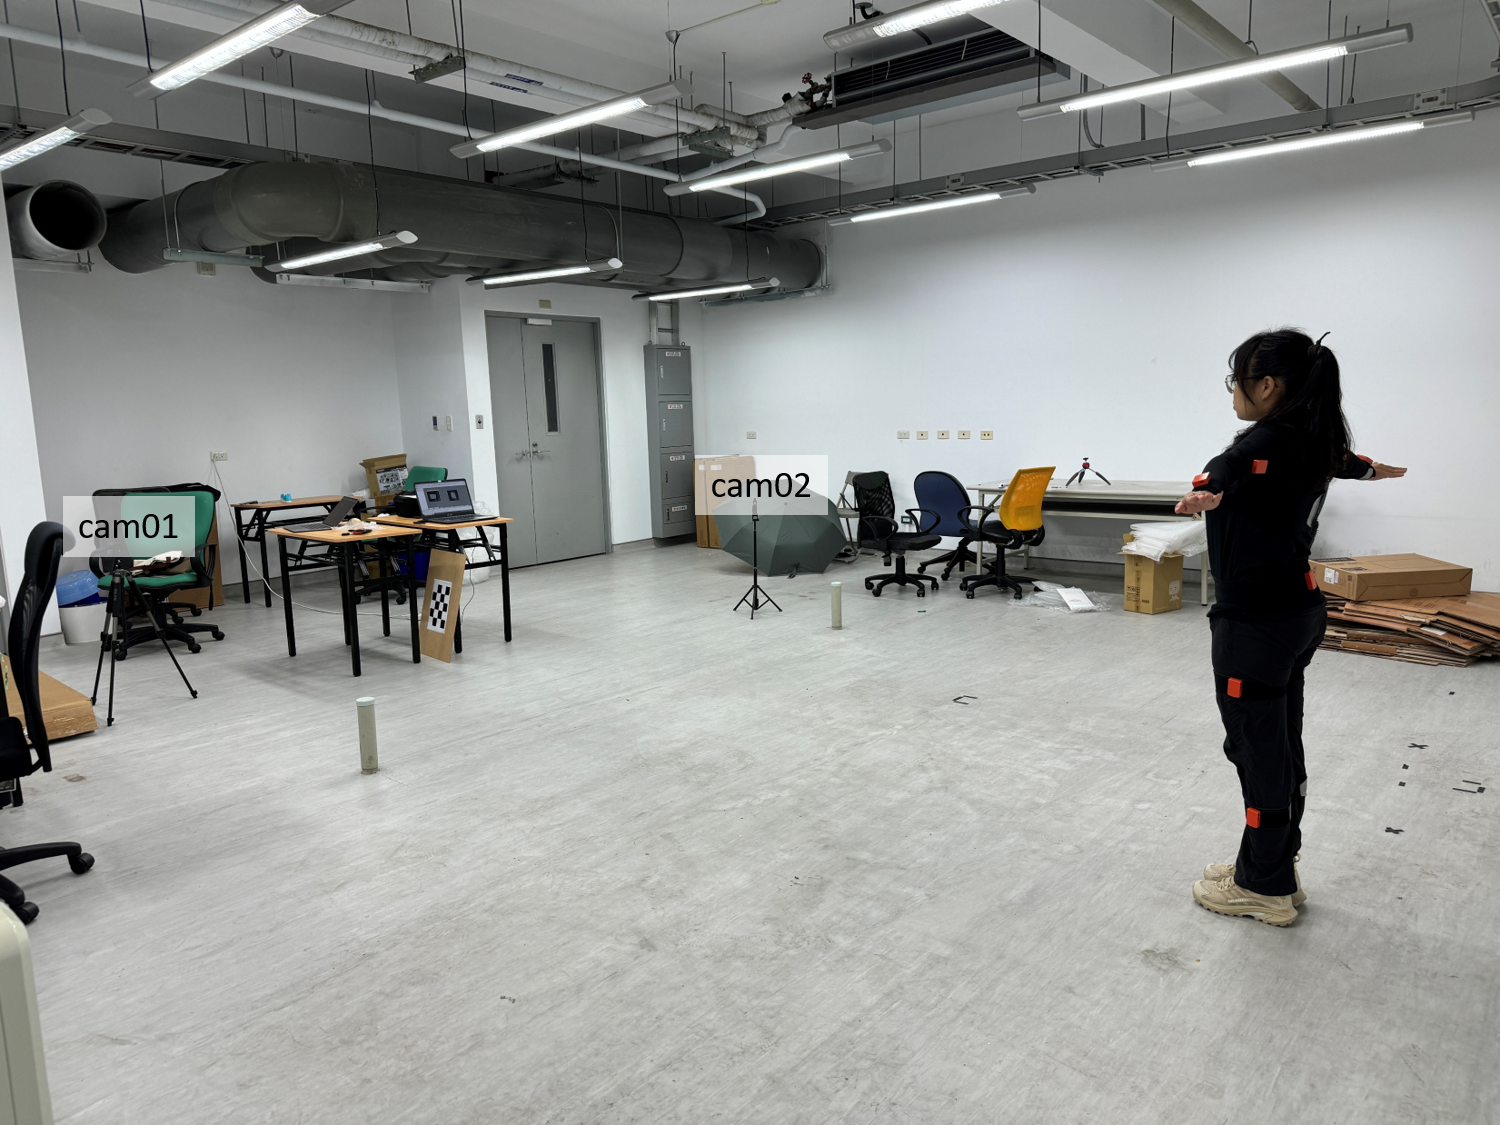
\includegraphics[width=.95\linewidth]{figure/ch3_fig_indoor_position2.png}
      \caption*{(b)相機與受試者位置 (後視)}
   \end{minipage}%
   \caption[實際實驗環境及相機與受試者位置]{實際實驗環境及相機與受試者位置}
   \label{ch3_fig_indoor_position}
\end{figure}

\clearpage

% \subsection{室外實驗環境及尺寸}
% % 室外實驗環境介紹
% % 這邊可以放一張室外實驗環境的照片
% 所有房間尺寸、活動範圍尺寸、相機位置和高度

\subsection{實驗系統設定}
% 系統架設介紹
本研究用於量測人體姿態的工具包含兩台 iPhone 手機、Xsens、棋盤格校正板。
兩台手機用於記錄人體姿態的影像資料,擺放於固定位置、固定角度,拍攝受試者的全身影像;
Xsens 用於記錄人體各肢段及棋盤格校正板的朝向資訊,共使用 10+1 顆 IMU 進行量測;
棋盤格校正板用於進行相機校正,取得相機內部參數及外部參數,以建立影像座標系與全域座標系間的關係。
另外,需要求受試者穿著黑色長袖上衣及黑色長褲,長度盡可能遮蓋住手腕及腳踝。


\subsubsection{位置資訊量測工具 - 相機及擺放位置}
本研究使用兩支 iPhone 手機進行影像資料蒐集,分別為 iPhone XR 及 iPhone 15 Pro,
iPhone XR 使用主鏡頭進行拍攝,焦距 26 (mm),光圈 ƒ/1.8,iPhone 15 Pro 使用主鏡頭進行拍攝,焦距 24 (mm),光圈 ƒ/1.78,
兩支手機皆設定影像擷取畫面為 1920x1080,幀率設定為 60 Hz。

本研究將 iPhone XR 編號為 cam01,將 iPhone 15 Pro 編號為 cam02,
手機擺放位置為圖~\ref{ch3_fig_indoor_scale} 中紅色圓點處,cam01 拍攝高度為 79 (cm),cam02 拍攝高度為 74 (cm),
cam 01 的拍攝視角為圖~\ref{ch3_fig_indoor_scale} 中綠色範圍,cam 02 的拍攝視角為圖~\ref{ch3_fig_indoor_scale} 中藍色範圍,
在實驗資料蒐集過程中,拍攝角度及位置皆維持不變。

\subsubsection{朝向資訊量測工具 - Xsens}
本研究使用 Xsens 提供之硬體 Awinda 及軟體 MT-manager 作為量測姿態朝向的工具,採樣率設定為 60 Hz,共使用 10+1 顆 IMU 進行量測,
十顆 IMU 分別黏貼於左右上臂中段外側、左右手腕外側、胸骨、骨盆、左右大腿中段外側、左右小腿中段外側,共十處,
如圖~\ref{ch3_fig_humanimu} 所示,分別為前視、左視、後視、右視時可看到的 IMU 位置, IMU 長軸 (即 x 軸) 與骨頭長度方向對齊,隨時間進行蒐集各時間點受試者各肢段的朝向資訊。
另一顆 IMU 黏貼於棋盤格校正板,量測棋盤格校正板的初始朝向,用以轉換影像座標系至全域座標系,如圖~\ref{ch3_fig_imgimu} 所示,IMU 的 x、y 軸方向對齊棋盤格校正板的 x、y 座標方向。

\begin{figure}[!ht]
   \centering
   \begin{minipage}{.25\textwidth}
     \centering
     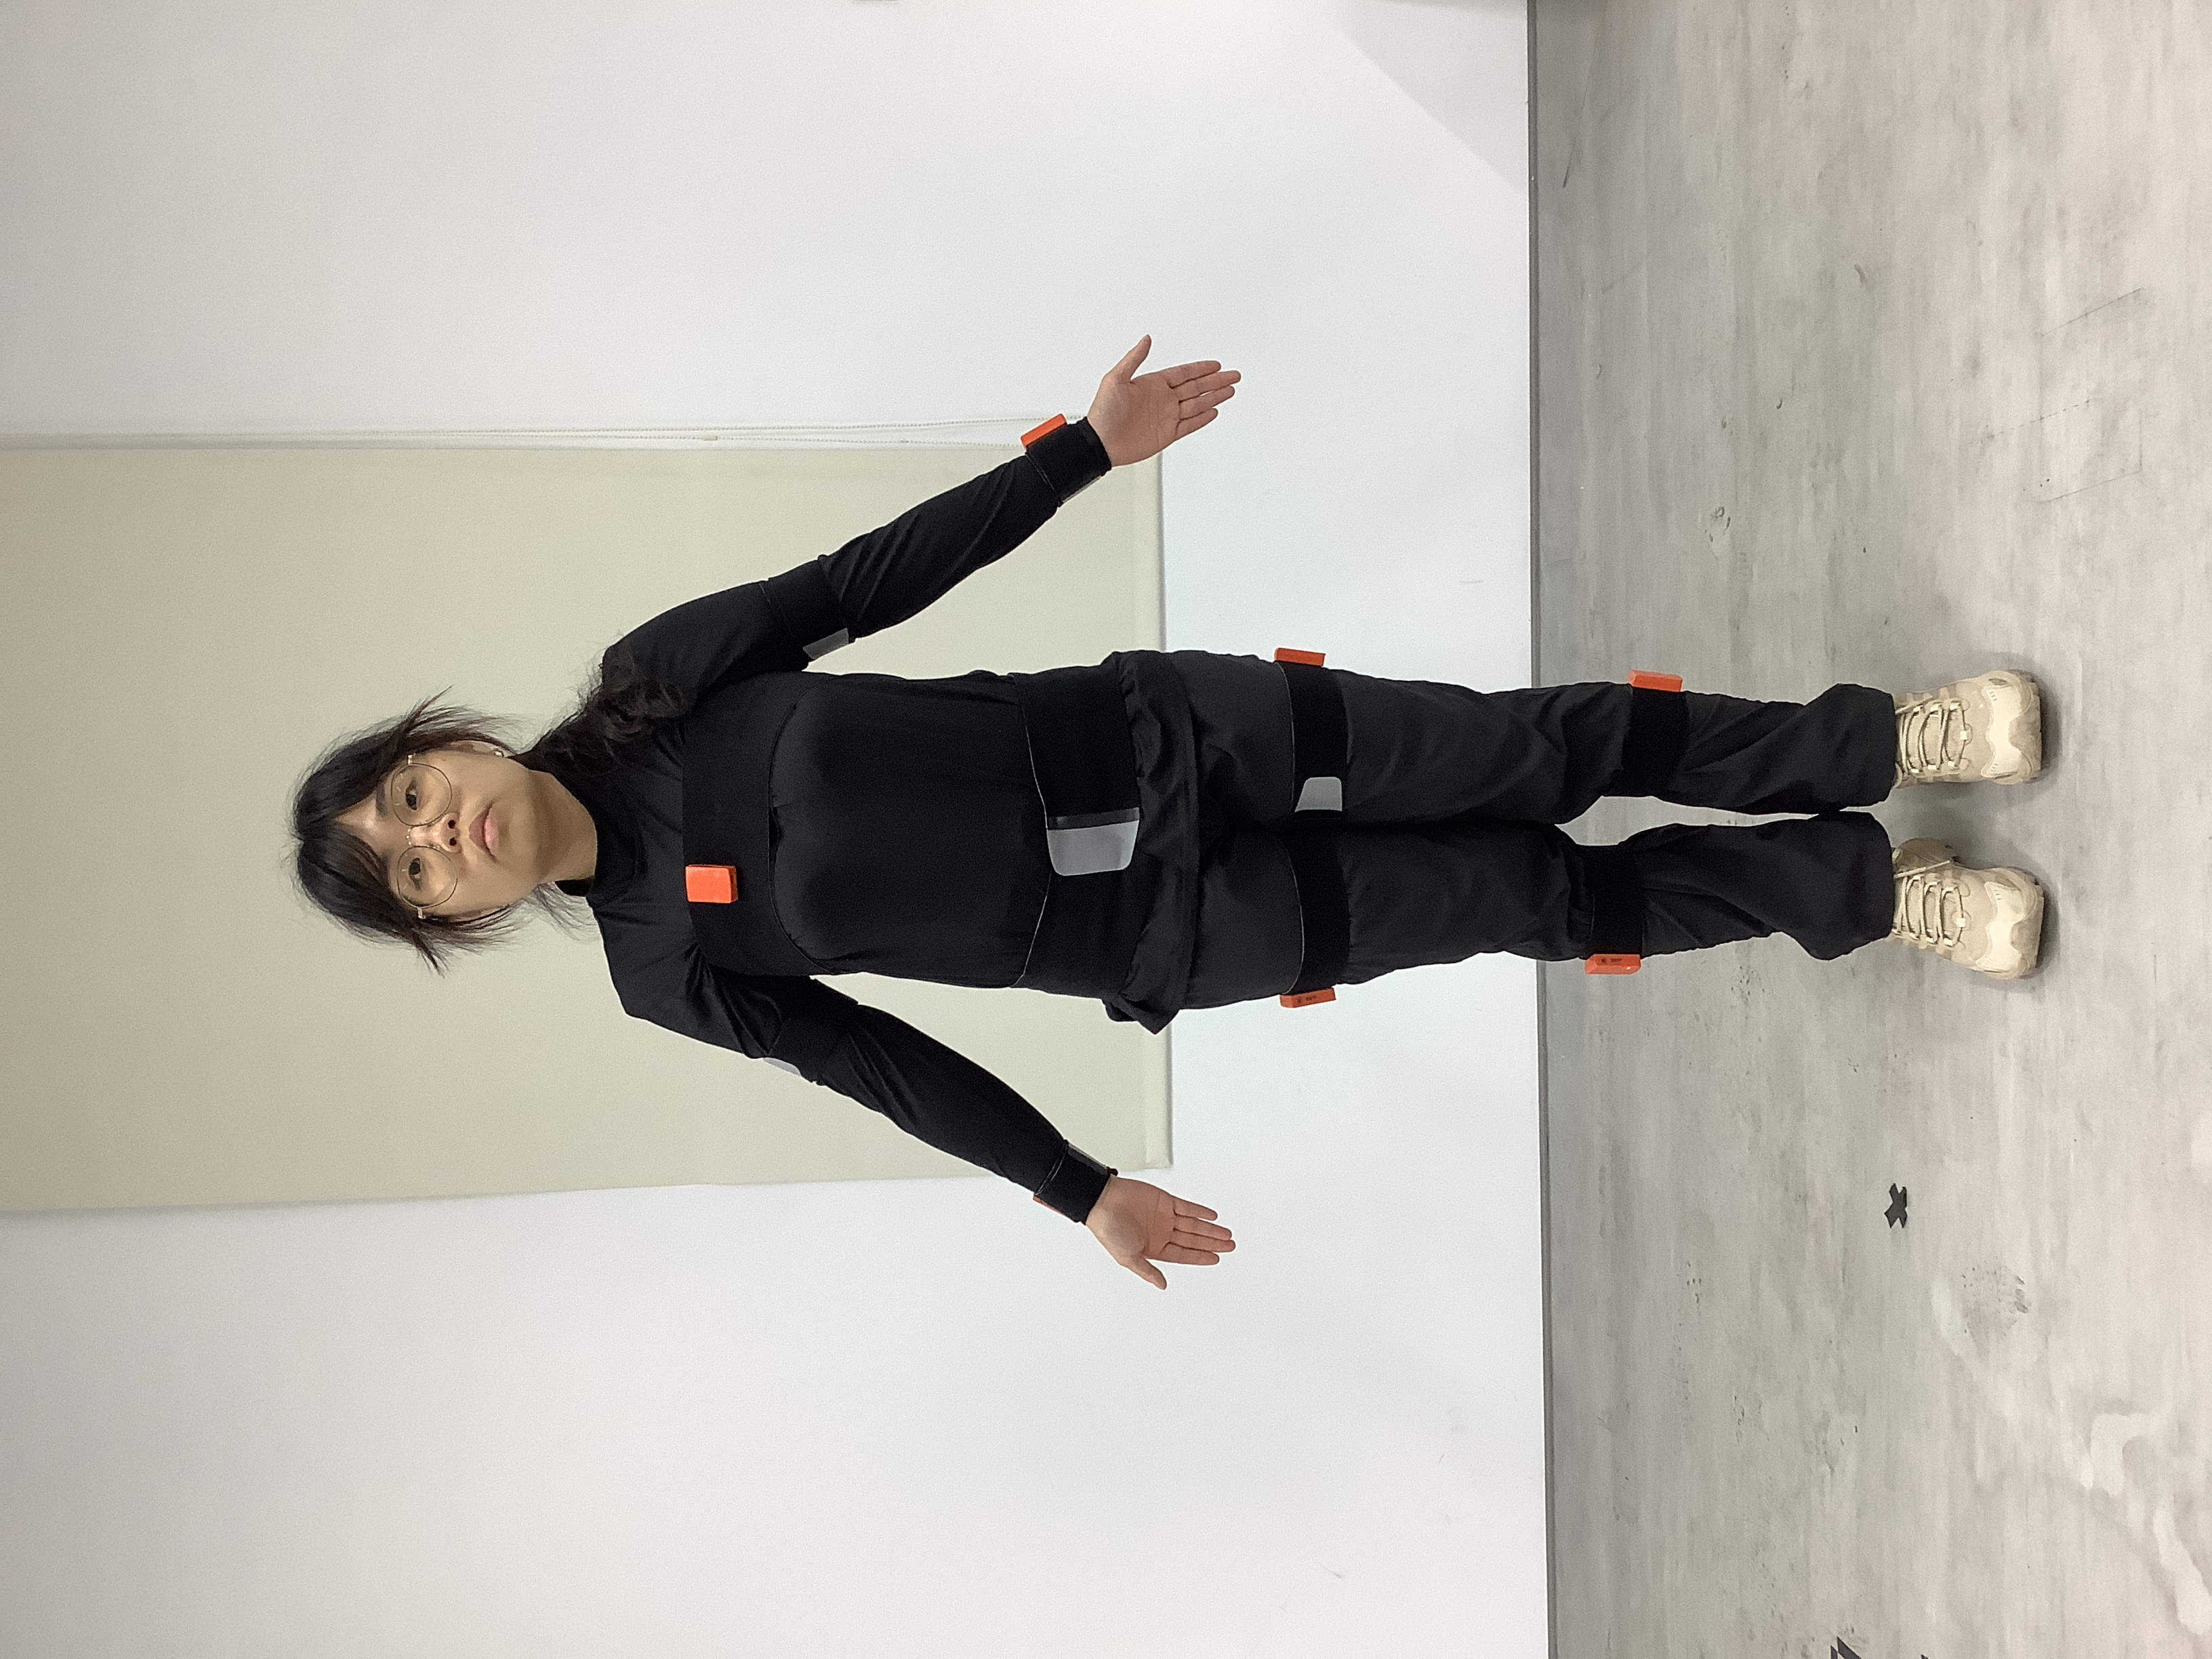
\includegraphics[width=.95\linewidth]{figure/ch3_fig_frontimu.JPG}
     \caption*{(a) 前視}
   \end{minipage}%
   \begin{minipage}{.25\textwidth}
      \centering
      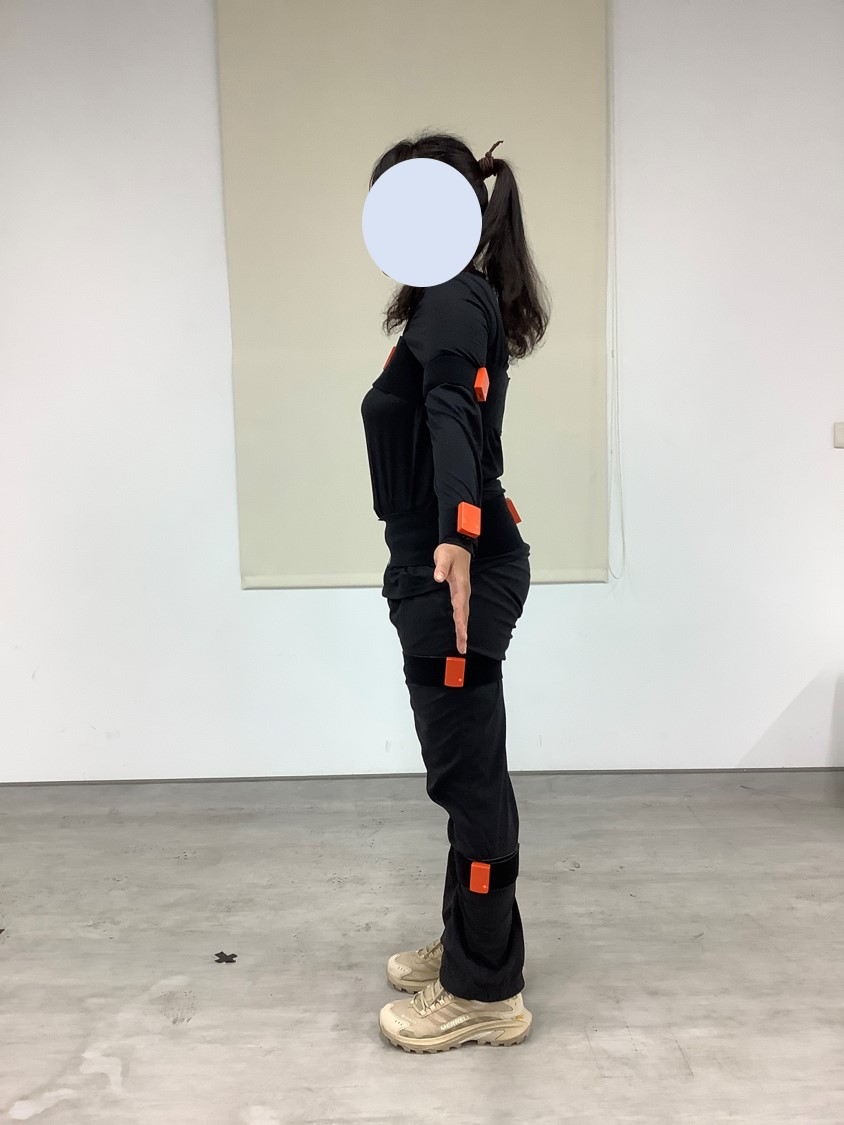
\includegraphics[width=.95\linewidth]{figure/ch3_fig_leftimu.JPG}
      \caption*{(b) 左視}
   \end{minipage}%
   \begin{minipage}{.25\textwidth}
      \centering
      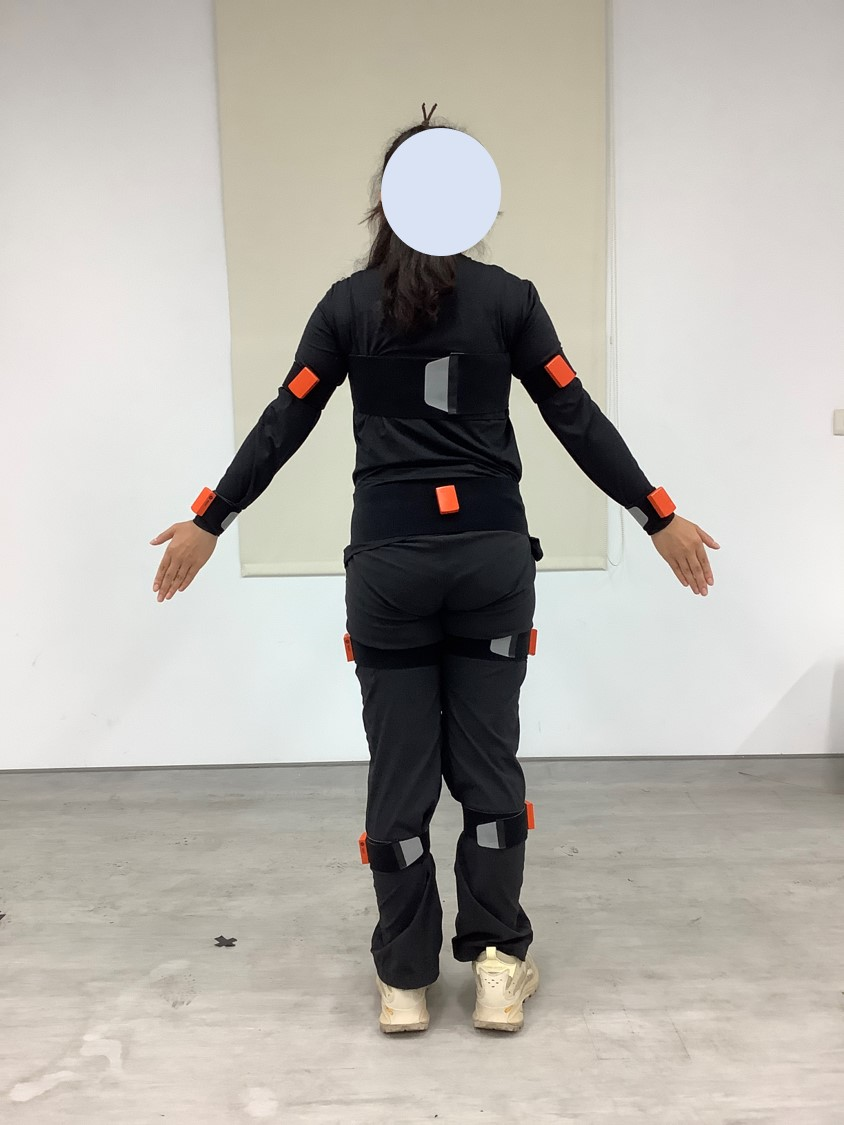
\includegraphics[width=.95\linewidth]{figure/ch3_fig_backimu.JPG}
      \caption*{(c) 後視}
   \end{minipage}%
   \begin{minipage}{.25\textwidth}
     \centering
     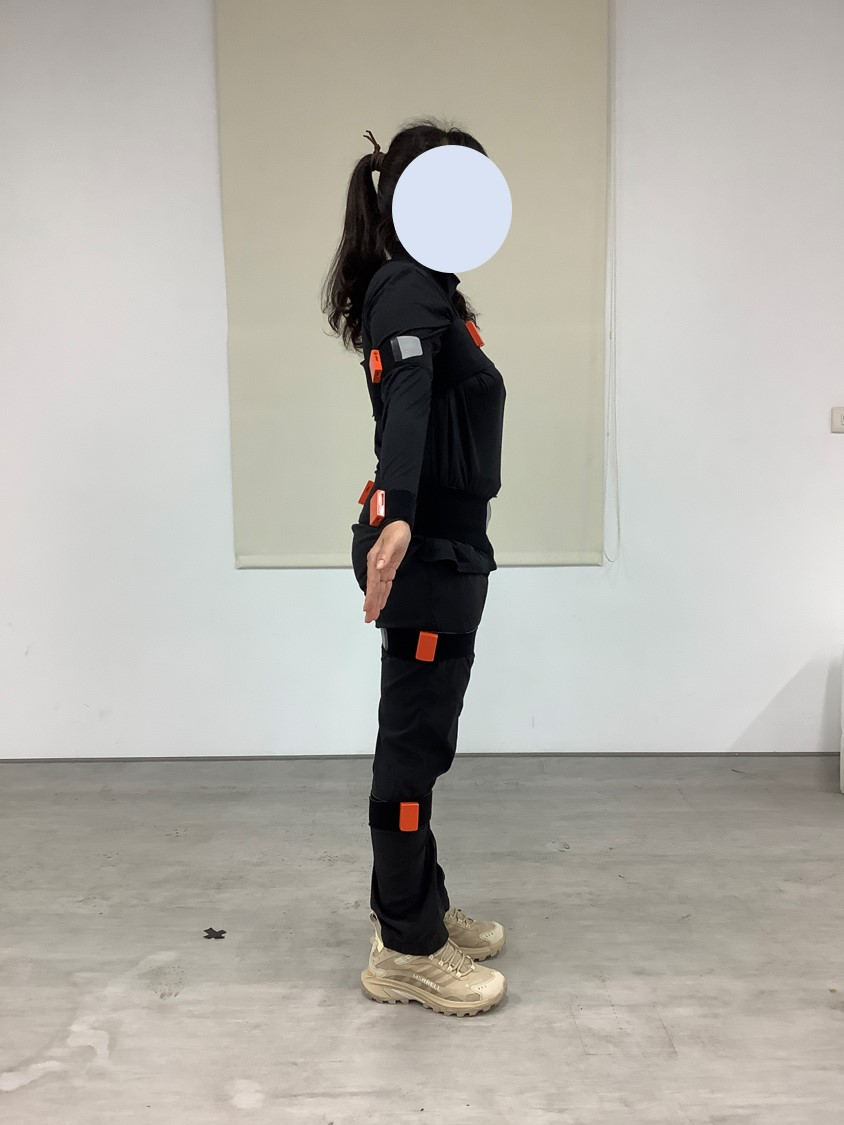
\includegraphics[width=.95\linewidth]{figure/ch3_fig_rightimu.JPG}
     \caption*{(d) 右視}
   \end{minipage}
   \caption[IMU 於人體黏貼位置及方向]{IMU 於人體黏貼位置及方向}
   \label{ch3_fig_humanimu}
\end{figure}

\begin{figure}[!ht]
   \centering
   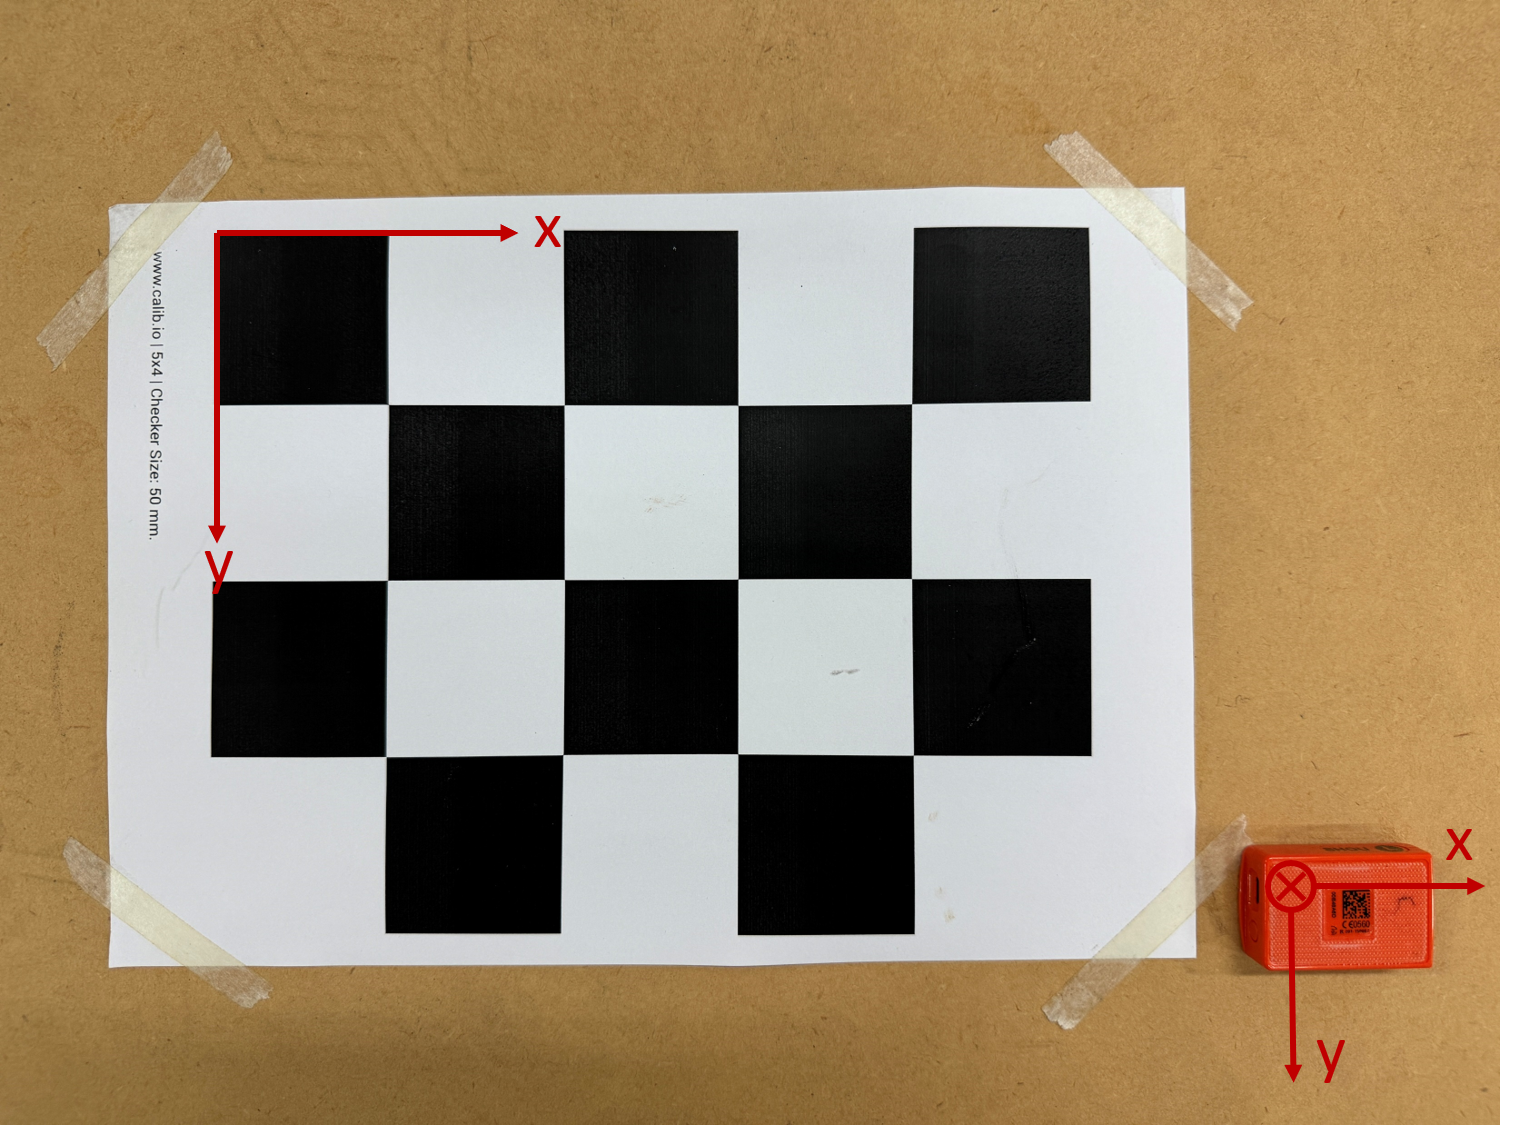
\includegraphics[width=8cm]{figure/ch3_fig_imgimu.png}
    \caption[IMU 於棋盤格校正板黏貼位置及方向]{IMU 於棋盤格校正板黏貼位置及方向}
    \label{ch3_fig_imgimu}
\end{figure}

\subsection{實驗動作}
% 實驗動作介紹
\subsubsection*{T-pose}
量測 T-pose 動作時,受試者面對相機,維持 T-pose 動作,這項動作特點為無任何動作變化,且無任何關節點被遮擋。
    
\subsubsection*{雙手握固定長度的桿子進行蹲站}
量測雙手握住固定長度的桿子進行蹲站動作時,受試者面對相機,雙手握住固定長度的桿子蹲下、起立、抬起雙手超過頭頂再蹲下為一循環,執行一個循環約耗時 3 秒,進行五個循環,這項動作的特點為動作有變化,在蹲下時關節點會受到遮擋。
    
\subsubsection*{開合跳}
量測開合跳動作時,受試者面對相機,進行開合跳動作,一次完整開合跳動作約耗時 2 秒,進行五次開合跳,這項動作的特點為動作變化快速,但無任何關節點受到遮擋。
    
\subsubsection*{折返跑}
量測折返跑動作時,受試者在動作場域內進行折返跑,跑到場地底端後蹲下摸地再起身往反方向跑,共進行五趟,這項動作的特點為受試者不面對鏡頭,動作有變化,且多關節點受到遮擋。
    
\subsubsection*{熱身運動}
量測熱身動作時,受試者在場域內進行腰部伸展、腿部拉筋等動作,這項動作的特點為整組動作包含正面、側面及背面的動作,且關節點會受到遮擋。
    
% \subsubsection*{組合動作}
% 組合動作為雙手握固定長度的桿子進行蹲站、開合跳、折返跑、熱身運動的連續動作,每種動作間會執行一次同步動作,這項組合動作的特點為包含多種變化速度的動作,且量測總時常較長

\subsection{量測實際四肢長度}
使用皮尺量測受試者的四肢長度,包含上肢長度、下肢長度,用以驗證感測器融合後的三維人體姿態估計結果。上、下肢量測方式皆為量測骨凸點間的距離,上肢上臂長度為肩關節至肘關節的距離,上肢前臂長度為肘關節至腕關節的距離,下肢大腿長度為髖關節至膝關節的距離,下肢小腿長度為膝關節至踝關節的距離,量測結果如表~\ref{ch3_limb_length} 所示。

\begin{table}[!ht]
   \caption[實際四肢長度]{實際四肢長度}
   \centering
   \label{ch3_limb_length}
   \setlength{\tabcolsep}{3pt}
   \renewcommand\arraystretch{1.5}
   \begin{tabular}{c|c|c|c|c}
      \toprule
       & 上臂 (mm) & 前臂 (mm) & 大腿 (mm) & 小腿 (mm) \\ 
      \midrule[2pt]
      右 & 307 & 215 & 375 & 360 \\
      左 & 295 & 211 & 365 & 365 \\
      \bottomrule
   \end{tabular}
\end{table}

% ------------------------- 3.3 ------------------------- %
\section{資料前處理}
% 資料前處理介紹
% 利用章節~\ref{ch3_exp_setting} 介紹的系統蒐集完實驗資料後,接下來將進行資料前處理,以利後續進行感測器融合。
% 資料前處理分為個人化人體模型建立、獲取骨盆中點位置、時間同步、空間校正四個部分,將於本章節進行討論。

\subsection{相機校正}
相機校正可視為影像世界和真實世界之間的轉換,其中包含外部參數 (Extrinsic Parameter) 及內部參數 (Intrinsic Parameter) 兩部分,透過相機校正計算公式~\ref{ch3_equ_camera_calibration},可以將全域座標系中的點 $(X, Y, Z)$ 轉換成在影像座標系中的點 $(u, v)$,如圖~\ref{ch3_fig_camera_calibration} 所示,將在全域座標系 (global coordinate system, g) 中的點 $P_g$,經過特定的旋轉、平移轉換及投影後,就可以轉換成影像座標系 (image coordinate system, img) 中的點 $P_{img}$。

相機校正技術發展至今,已有許多開源軟體可供使用,如 OpenCV~\cite{opencv_library}、MATLAB Camrea Calibration Toolbox,也有許多學者對 OpenCV 進行改良,提出更為方便易上手的相機校正工具,如 Pose2Sim ~\cite{Pagnon_2022_JOSS}~\cite{Pagnon_2021_Robustness}~\cite{Pagnon_2022_Accuracy},本研究即使用 Pose2Sim 提供的相機校正工具,計算出相機內部參數及外部參數。後續將使用相機內部參數及外部參數進行影像座標系與全域座標系的轉換、感測器融合、三角測量計算等工作。

\begin{equation}
   s
   \begin{bmatrix}
      u \\ v \\ 1
   \end{bmatrix}
   =
   \begin{bmatrix}
      \alpha_x & s & u_o \\
      0 & \alpha_y & v_o \\
      0 & 0 & 1 \\
   \end{bmatrix}
   \begin{bmatrix}
      r_{11} & r_{12} & r_{13} & t_{1} \\
      r_{21} & r_{22} & r_{23} & t_{2} \\
      r_{31} & r_{32} & r_{33} & t_{3} \\
   \end{bmatrix}
   \begin{bmatrix}
      X \\
      Y \\
      Z \\
      1 \\
   \end{bmatrix}
   \label{ch3_equ_camera_calibration}
\end{equation}

\begin{figure}[!ht]
   \centering
   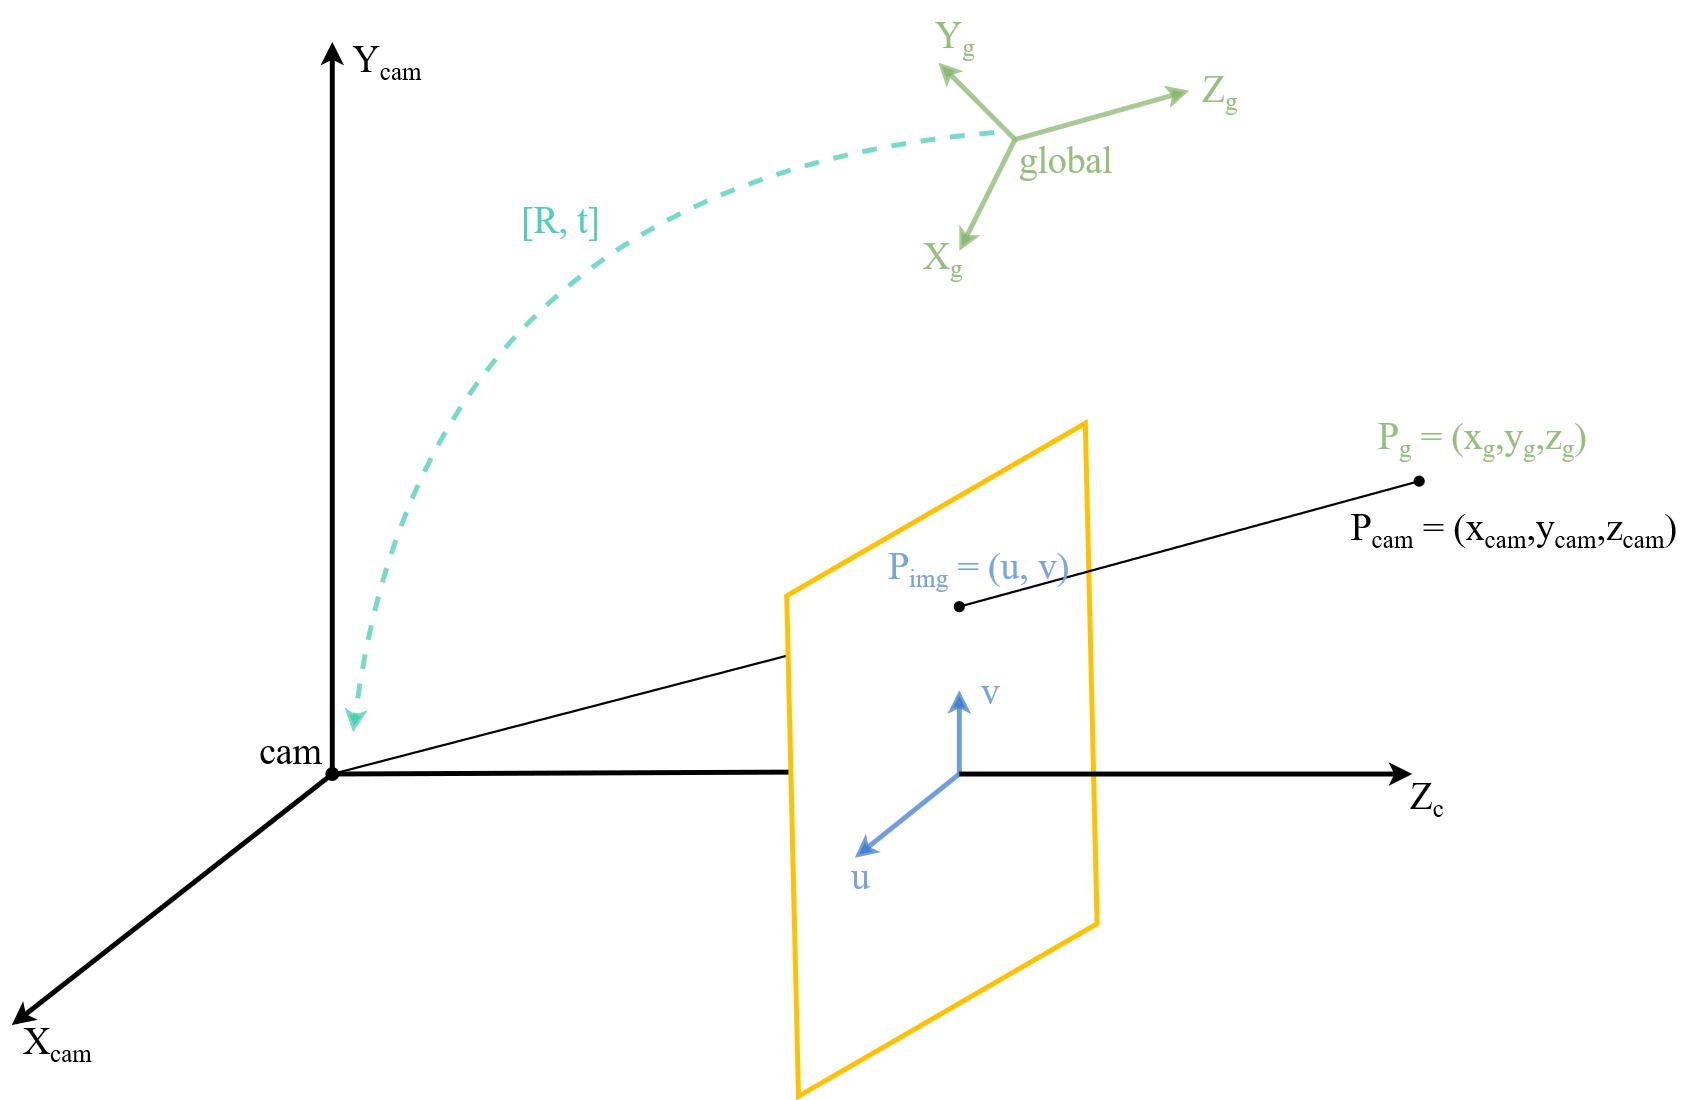
\includegraphics[width=\linewidth]{figure/ch3_fig_camera_calibration.png}
    \caption[相機校正座標系~\cite{dehkharghani2014geometric}]{相機校正座標系~\cite{dehkharghani2014geometric}}
    \label{ch3_fig_camera_calibration}
\end{figure}

\subsubsection*{外部參數}
如圖~\ref{ch3_fig_camera_calibration},
假設有一在原點為校正板左上角的全域座標系 (global coordinate system, g) 中的點 $P_g$,
將 $P_g$ 經過特定的旋轉及平移轉換後,就可以轉換成以相機焦點為原點的相機座標系 (camera coordinate system, cam) 中的點 $P_{cam}$,
這個特定的旋轉及平移轉換即為相機的外部參數,旋轉以一個 3$\times$3 的旋轉矩陣 $R$ 表示,平移以一個 3$\times$1 的平移向量 $T$ 表示,
因為在矩陣計算上,世界座標會先經過旋轉再平移,因此平移向量 $T$ 會經過旋轉矩陣 $R$ 的作用,形成 $RT$,
再將 $[R|RT]$ 合併成一個 3$\times$4 的外部參數矩陣 $[R|RT]$,
即為式~\ref{ch3_equ_camera_calibration}中,等號右邊第二項。

\subsubsection*{內部參數}
將在相機座標系中的點 $P_{cam}$ 經過投影、平移及幾何校正,轉換成在影像座標系 (image coordinate system) 中的點為 $P_{img}$,
為圖~\ref{ch3_fig_camera_calibration}中,將 $P_{cam}$ 轉換至 $P_{img}$ 的過程,
這個投影、平移及幾何校正的過程即為相機的內部參數,為一個 3$\times$3 的矩陣,
即為式~\ref{ch3_equ_camera_calibration}中,等號右邊第一項,
內部參數包含焦距、影像座標系的圓點位置、解析度、 pixel 夾角等參數,
由於這些參數皆與相機內部的硬體參數有關,因此稱為相機內部參數。

\subsection{以影像辨識方法建立個人化三維人體模型}\label{ch3_skeleton_method}
% 個人化三維人體模型建立介紹
% 伸縮沒有寫到,要怎麼加進去?
% TODO:覺得可以把我為甚麼選擇用 OpenPose 不用 mediapipe 寫在這邊
為方便將影像資訊與 IMU 資訊融合,需將 IMU 的朝向資訊轉換成以座標點為描述方式的人體姿態,
因此需透過一個以關節座標點為描述方式的三維人體模型,將人體肢段向量與 IMU 朝向資訊相乘,即可得到人體各關節點在活動過程中的位置資訊。

在文獻~\cite{Zhang_2020_CVPR} 中,作者使用 Vicon 系統提供的三維人體模型,並以其為基礎,將 IMU 的朝向資訊轉換成以座標點為描述方式的人體姿態,
其中,Vicon 系統建立出的三維人體模型為預定義的運動學模型,藉由量測過程中的標記點取得受試者的四肢長度,
以量測長度進行運動學模型的縮放,成為個人化的三維人體模型,但是在非實驗室的環境中無法使用 Vicon 進行量測,進而取得三維人體模型,
因此本研究透過 Pose2Sim ~\cite{Pagnon_2022_JOSS}~\cite{Pagnon_2021_Robustness}~\cite{Pagnon_2022_Accuracy} 提出之方法,
使用影像辨識技術,辨識每一視角中人體的關節點在影像中的位置,並利用相機校正技術建立出每一關節在空間中的位置,以此方式建立個人三維人體模型。

% 章節~\ref{ch4_skeleton_exp} 將會利用 TotalCapture Dataset~\cite{Trumble:BMVC:2017}提供的影像資料,進行影像辨識與三角測量計算,
% 並將結果與 TotalCapture Dataset 提供之 Vicon 三維人體模型比對,以驗證此方法的可行性。

\subsubsection{建立方法}
% 影像辨識
% 這邊好像跟第四章的4.1.1有點重複,如果這邊和4.1都要留的話可能就要把下一節的結果與驗證搬到4.1那邊
% 這邊就只要簡單介紹一下方法就好,然後這邊可以應該可以把為何要選 OpenPose 不選 mediapipe 也寫上去
% 只是這樣的話就要想一下4.1.2的實驗執行要怎麼寫(不然如果真的想不到可能就要刪掉實驗執行這塊,畢竟也只是 run 而已),
% 4.1.1的應該可以寫用了哪些數據
% 考慮要不要寫為何選擇使用 OpenPose 不選 mediapipe,要寫的話可以寫在這一段的開頭
本方法流程如圖~\ref{ch3_fig_skeleton_flow} 所示。
以 T-pose 的姿勢拍攝影片後,進入後續軟體端處理流程。

\begin{figure}[!ht]
   \centering
   
\includegraphics[width=\linewidth]{figure/ch3_fig_skeleton_flow.png}
    \caption[個人化三維人體模型建立流程圖]{個人化三維人體模型建立流程圖}
    \label{ch3_fig_skeleton_flow}
\end{figure}

首先,使用 OpenPose~\cite{8765346}~\cite{wei2016cpm}~\cite{simon2017hand}~\cite{cao2017realtime}
影像辨識技術辨識每一視角人體關節點在影像中的位置(使用 BODY-25B model),辨識結果如圖~\ref{ch3_fig_OpenPose_result} 所示,其可辨識出左右肩膀、左右手肘、左右手腕、左右骨盆、左右膝蓋、左右腳踝等關節位置,
% 圖~\ref{ch3_fig_OpenPose_result} (a) 為
% 其可辨識出左右肩膀、左右手肘、左右手腕、左右骨盆、左右膝蓋、左右腳踝等關節位置,如圖~\ref{ch3_fig_OpenPose} 所示;
接著,利用棋盤格方法之相機校正技術計算出各個相機的內部參數及外部參數;
再來,利用方才相機校正之結果,經由三角測量計算建立出關節在空間中的位置,並使用距離公式計算每一關節之間的距離;
最後,基於 TotalCapture Dataset ~\cite{Trumble:BMVC:2017} 提供之 Vicon 三維人體模型,利用計算出的距離進行三維人體模型伸縮,得到與受試者四肢、身高相似之個人化三維人體模型,如圖~\ref{ch3_fig_my_skeleton},圖中有四種顏色分別代表四肢,紅色為右腿,兩個座標點分別代表右膝蓋及右腳踝,黃色為左腿,兩個座標點分別代表左膝蓋及左腳踝,藍色為右手兩個座標點分別代表右手肘及右手腕,紫色為左手,兩個座標點分別代表左手肘及左手腕。

\begin{figure}[!ht]
   \centering
   \begin{minipage}{.5\textwidth}
     \centering
     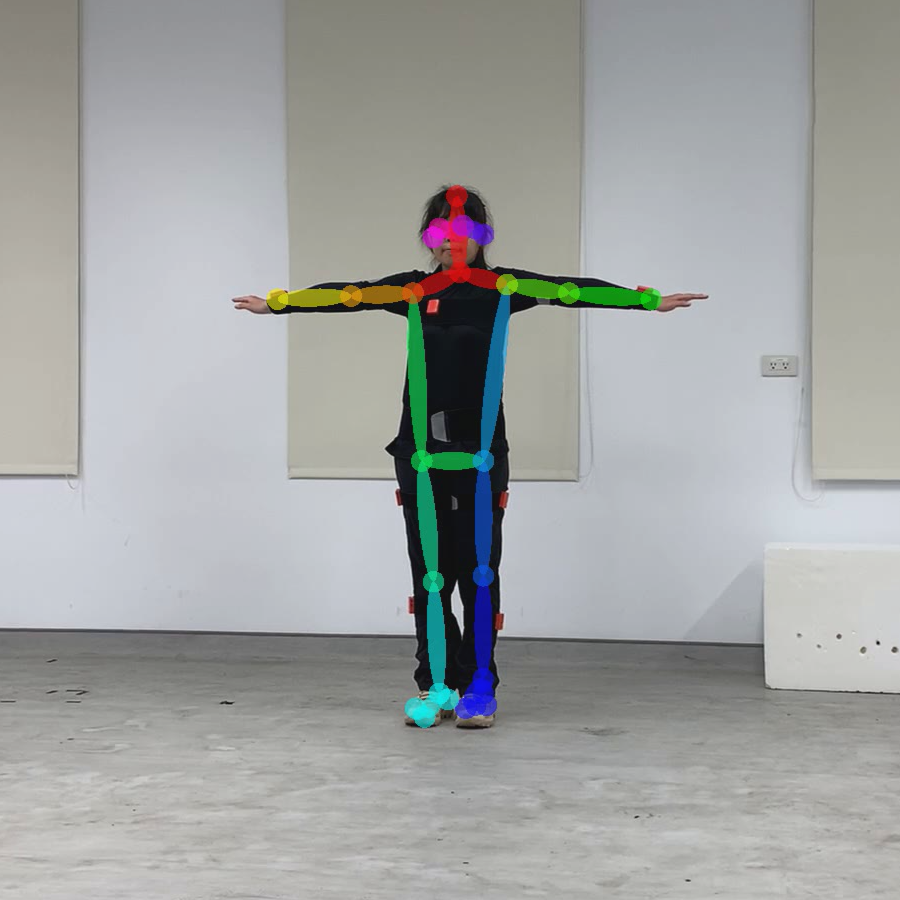
\includegraphics[width=.95\linewidth]{figure/ch3_fig_OpenPose_result_cam01.png}
     \caption*{(a) cam01}
   \end{minipage}%
   \begin{minipage}{.5\textwidth}
      \centering
      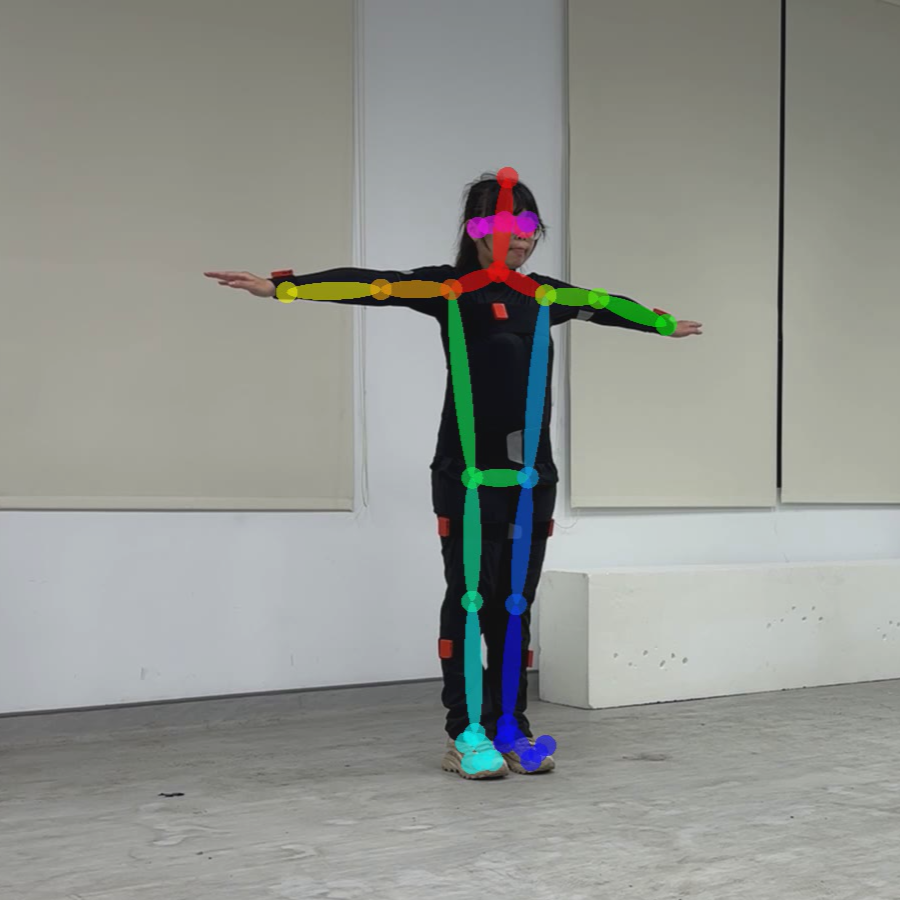
\includegraphics[width=.95\linewidth]{figure/ch3_fig_OpenPose_result_cam02.png}
      \caption*{(b) cam02}
   \end{minipage}
   \caption[OpenPose 辨識結果]{OpenPose 辨識結果}
   \label{ch3_fig_OpenPose_result}
\end{figure}

% \begin{figure}[!ht]
%    \centering
%    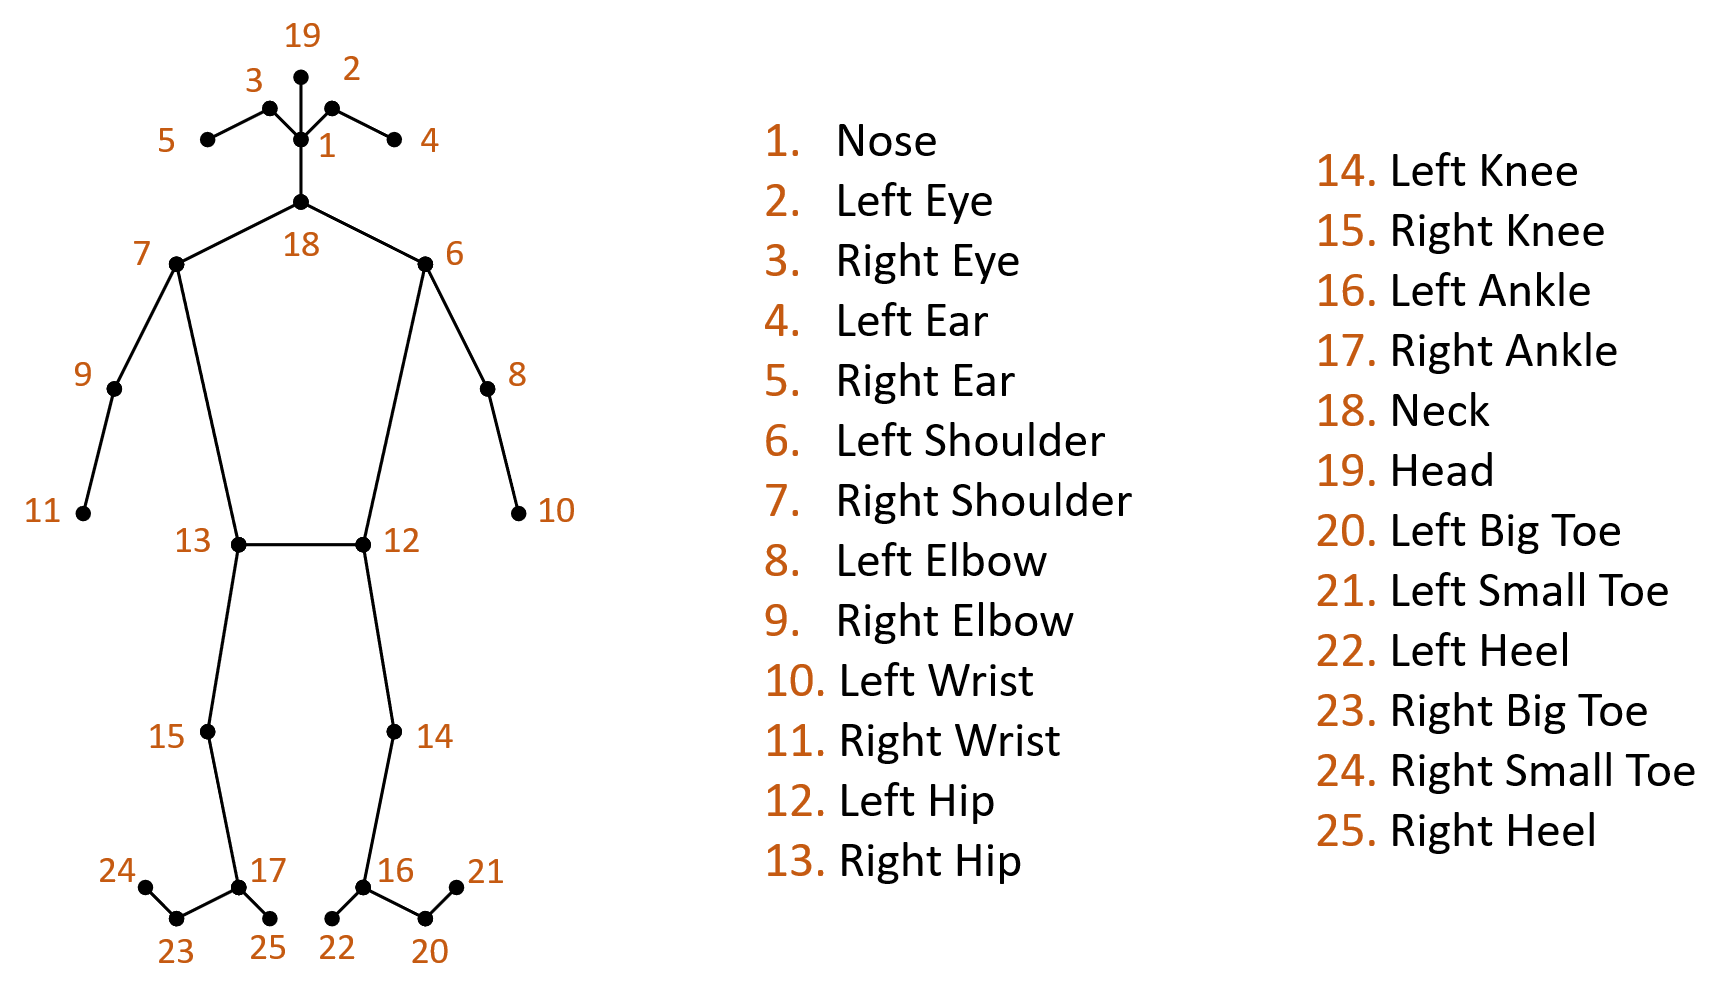
\includegraphics[width=\linewidth]{figure/ch3_fig_OpenPose.png}
%     \caption[OpenPose 關節點對應位置]{OpenPose 關節點對應位置}
%     \label{ch3_fig_OpenPose}
% \end{figure}

\begin{figure}[!ht]
   \centering
   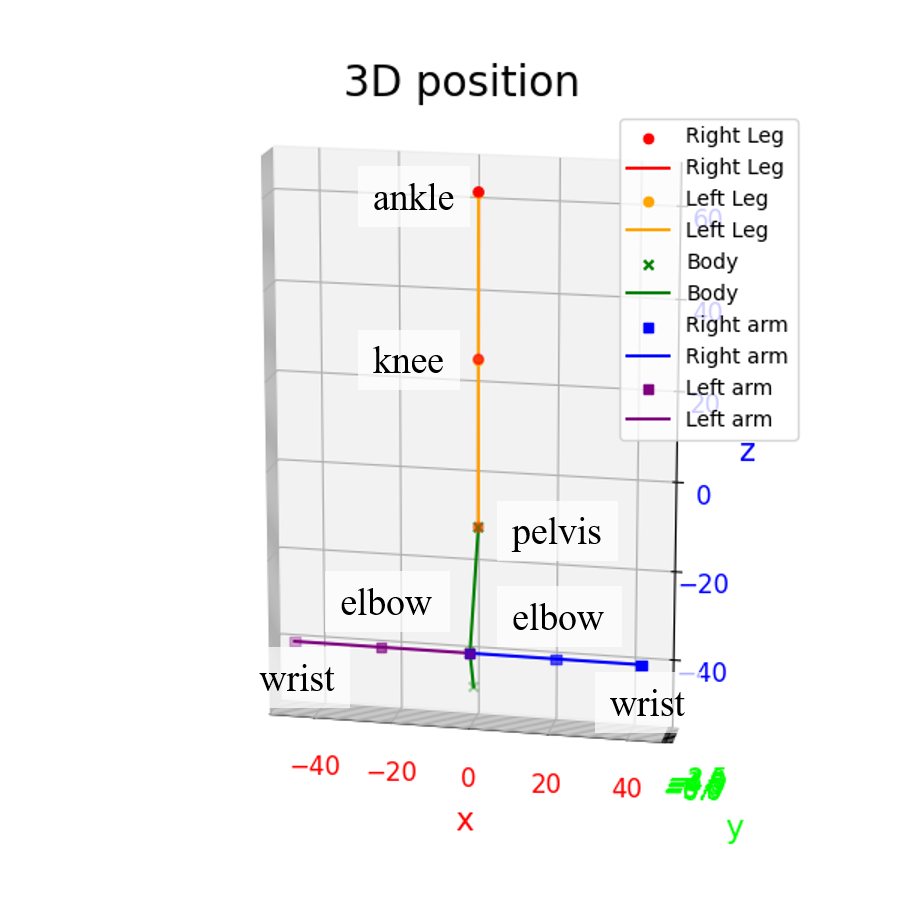
\includegraphics[width=8cm]{figure/ch3_fig_my_skeleton.png}
   \caption[個人化三維人體模型建立結果]{個人化三維人體模型建立結果}
   \label{ch3_fig_my_skeleton}
\end{figure}

\subsubsection{應用}
% FIXME:加圖
現階段建立出的三維人體模型僅用於後續感測器融合的過程中,將 IMU 的朝向資訊轉換成以座標點為描述方式的人體姿態,經由旋轉矩陣可利用 IMU 的朝向資訊,將初始三維人體模型的每一對應肢段向量進行旋轉,得到受試者在活動過程中的人體姿態。

\clearpage

\subsection{計算骨盆在影像坐標系中的位置}
% 軟體介紹;OpenPose
% OpenPose 為一款
% 由  Ginés Hidalgo, Zhe Cao, Tomas Simon, Shih-En Wei, Yaadhav Raaj, Hanbyul Joo, and Yaser Sheikh 等人開發的開源軟體,
% 為第一個在單個圖像上可以同時偵測人體關節、手部關節、面部表情和足部關鍵點(總共 135 個關鍵點)的實時多人偵測系統,
% 其可於 Windows、MacOS、Ubuntu 等作業系統上執行,並支援 Python、C++ 等程式語言,
% 輸入資源包括圖片、影像、網路攝影機等,
% 並可輸出原始影像加關鍵點顯示的疊圖 (PNG,JPG,AVI,...),
% 或是輸出純文字檔案 (JSON,XML,YAML...),其中紀錄關鍵點相對於輸入圖像的像素座標位置及 0~1 的分數。
為減少影像辨識過程中的計算量及計算時間,在文獻~\cite{Zhang_2020_CVPR} 中,
作者使用相機校正的外部參數將 Vicon 系統所提供的骨盆三維量測數據投影至影像座標系中,
並以在影像座標系中的骨盆座標為中心,進行影像裁切,以減少後續影像辨識及感測器融合的計算量。

由於本研究無法使用 Vicon 系統進行量測,無法使用上述方式進行影像裁切,
因此本研究選擇以 OpenPose ,搭配其提供之 BODY\_25B 模型進行初步影像辨識,
辨識出每一幀照片中 25 個人體關鍵點在影像座標系中的位置,
% 可辨識出的關鍵點如圖~\ref{ch3_fig_OpenPose} 所示,
並計算左骨盆及右骨盆的中點在影像座標系中的位置,以此計算結果作為該張影像的中點進行影像裁切,減低後續影像辨識及感測器融合的計算量。

\subsection{時間同步}
% 時間軸同步介紹
本研究使用拍手~\cite{pons2012data} 的方法進行時間同步,在實驗動作開始及結束時,受試者皆需進行拍手動作,
動作流程為:兩手打直張開呈現 T-pose 維持 1 \textasciitilde\ 2 秒,然後迅速合攏雙手並拍手,最後維持合掌姿勢 1 \textasciitilde\ 2 秒。
透過拍手動作,可在影像資料的音軌中找到明顯的拍手聲音,
並在 IMU 資料中找到快速拍手動作的時間點,因為迅速合攏手掌的拍手動作會產生明顯加速度變化,
以此時間點作為時間同步的基準點,將影像資料及 IMU 資料進行時間同步,以確保兩者之間的時間軸一致。
在同步並剪輯影像資料及 IMU 資料時有一點需要注意,如圖~\ref{ch3_fig_timesyn} 所示,
同步兩種資訊時,由於加速度的明顯變化是發生在拍手那一刻的前後一幀,IMU 記錄到的最大加速度時刻會與拍手瞬間的前一幀相對應,
因此在裁切 IMU 資料時,需將拍手動作前後一幀的資料保留,確保拍手動作的加速度變化完整呈現,
進行影像剪輯時,需將合掌姿勢前後一個幀的影像資料保留,以確保拍手動作的完整呈現,且可與 IMU 資料同步。

\begin{figure}[!ht]
   \centering
   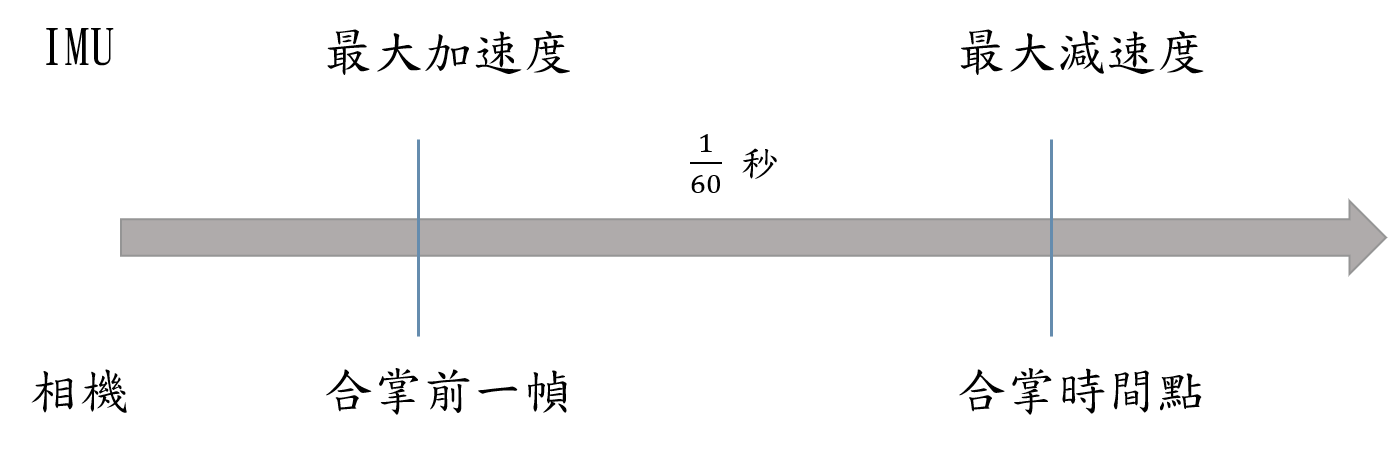
\includegraphics[width=11cm]{figure/ch3_fig_timesyn.png}
   \caption[時間同步方法]{時間同步方法}
   \label{ch3_fig_timesyn}
\end{figure}

\clearpage

\subsection{空間校正}
% 座標系轉換介紹
在人體量測領域中,每一量測方法都有其固有且常用的座標系,
因此在進行感測器融合時,必須將各感測器的座標系轉換至同一座標系,以方便後續感測器融合計算。
本研究共涉及六種座標系,可分為影像系統及 IMU 感測器系統兩大部分,兩部分的共同座標系為全域座標系 (global coordinate system, g)。
影像系統涉及三種座標系,分別為圖像座標系 (image coordinate system, img)、
相機座標系 (camera coordinate system, cam) 及全域座標系 (global coordinate system, g);
IMU 感測系統則涉及四種座標系,分別為人體模型座標系 (bone coordinate system, b)、感測器座標系 (sensor coordinate system, s)、
IMU local 座標系 (imu local coordinate system, i)、全域座標系 (global coordinate system, g)。
各座標系的定義及轉換關係將於以下進行介紹。

\subsubsection{座標系定義}
% 各座標系定義介紹
圖像座標系為二維座標系,如圖~\ref{ch3_fig_frame} (a) 所示,以圖像左上角為原點,x 軸沿圖像右側為延伸為正,y 軸沿圖像下側延伸為正;
相機座標系如圖~\ref{ch3_fig_frame} (b) 所示,以相機的光軸 0 點為原點,z 軸與光軸重和,指向相機前方為正, x 軸指向相機右方為正, y 軸指向相機下方為正;
人體模型座標系以 TotalCapture Dataset 提供之 Vicon 三維人體模型所在之座標系為基礎,如圖~\ref{ch3_fig_frame} (c) 所示,其以人體骨盆中心為原點, +x、+y、+z 方向分別為向右 (red)、向後 (green)、向下 (blue);
感測器座標系如圖~\ref{ch3_fig_frame} (d) 所示,以感測器本身為原點,
於 Xsens 系統中,定義其 x 軸為長邊延伸方向,y 軸為短邊延伸方向,z 軸則沿最大平面法向;
IMU local 座標系以感測器所在地為原點,y 軸沿子午線指向正北為正,z 軸指向天頂為正,x 軸與 yz 平面垂直,指向正東為正;
全域座標系以固定的全球基準點為原點 (例如地球中心),x 軸以磁北極為參考方向,z 軸參考方向與 IMU local 座標系 z 軸相同,指向天頂為正,
y 軸則以右手定則決定,通常指向西方為正。
座標系間的關係及旋轉矩陣將於下一段進行介紹。

\begin{figure}[!ht]
   \centering
   \begin{minipage}{.5\textwidth}
      \centering
      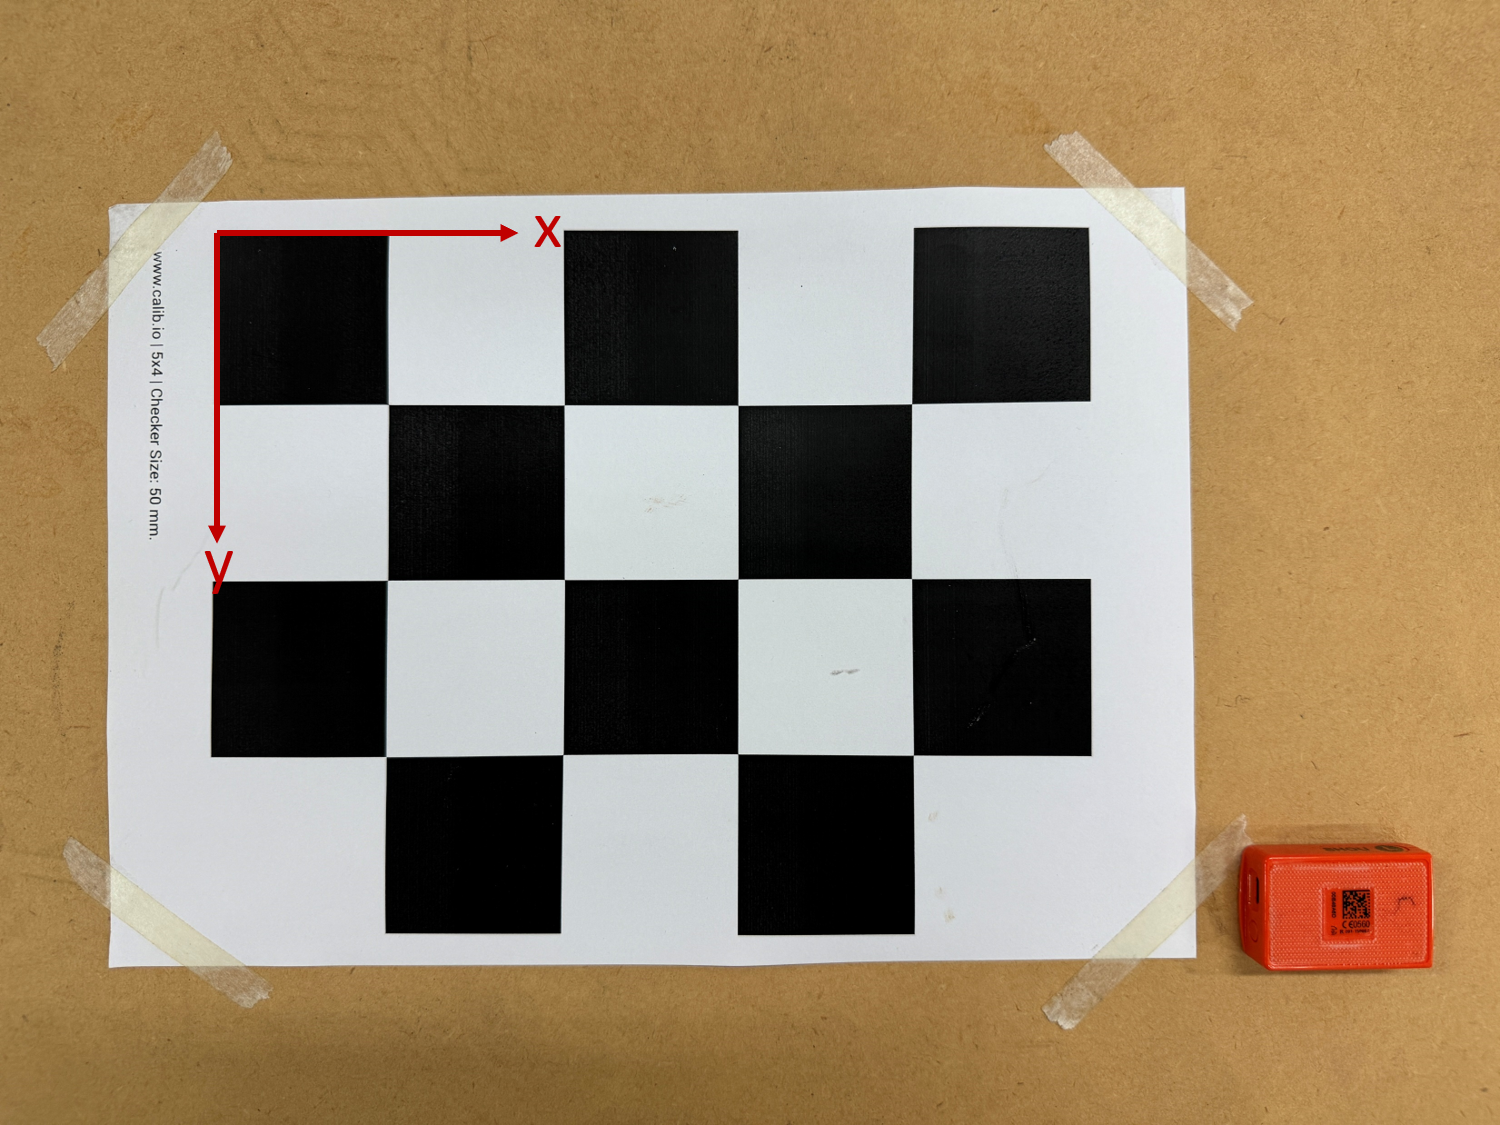
\includegraphics[width=.95\linewidth]{figure/ch3_fig_imgframe.png}
      \caption*{(a) 影像座標系}
   \end{minipage}%
   \vspace{5mm}%
   \begin{minipage}{.5\textwidth}
      \centering
      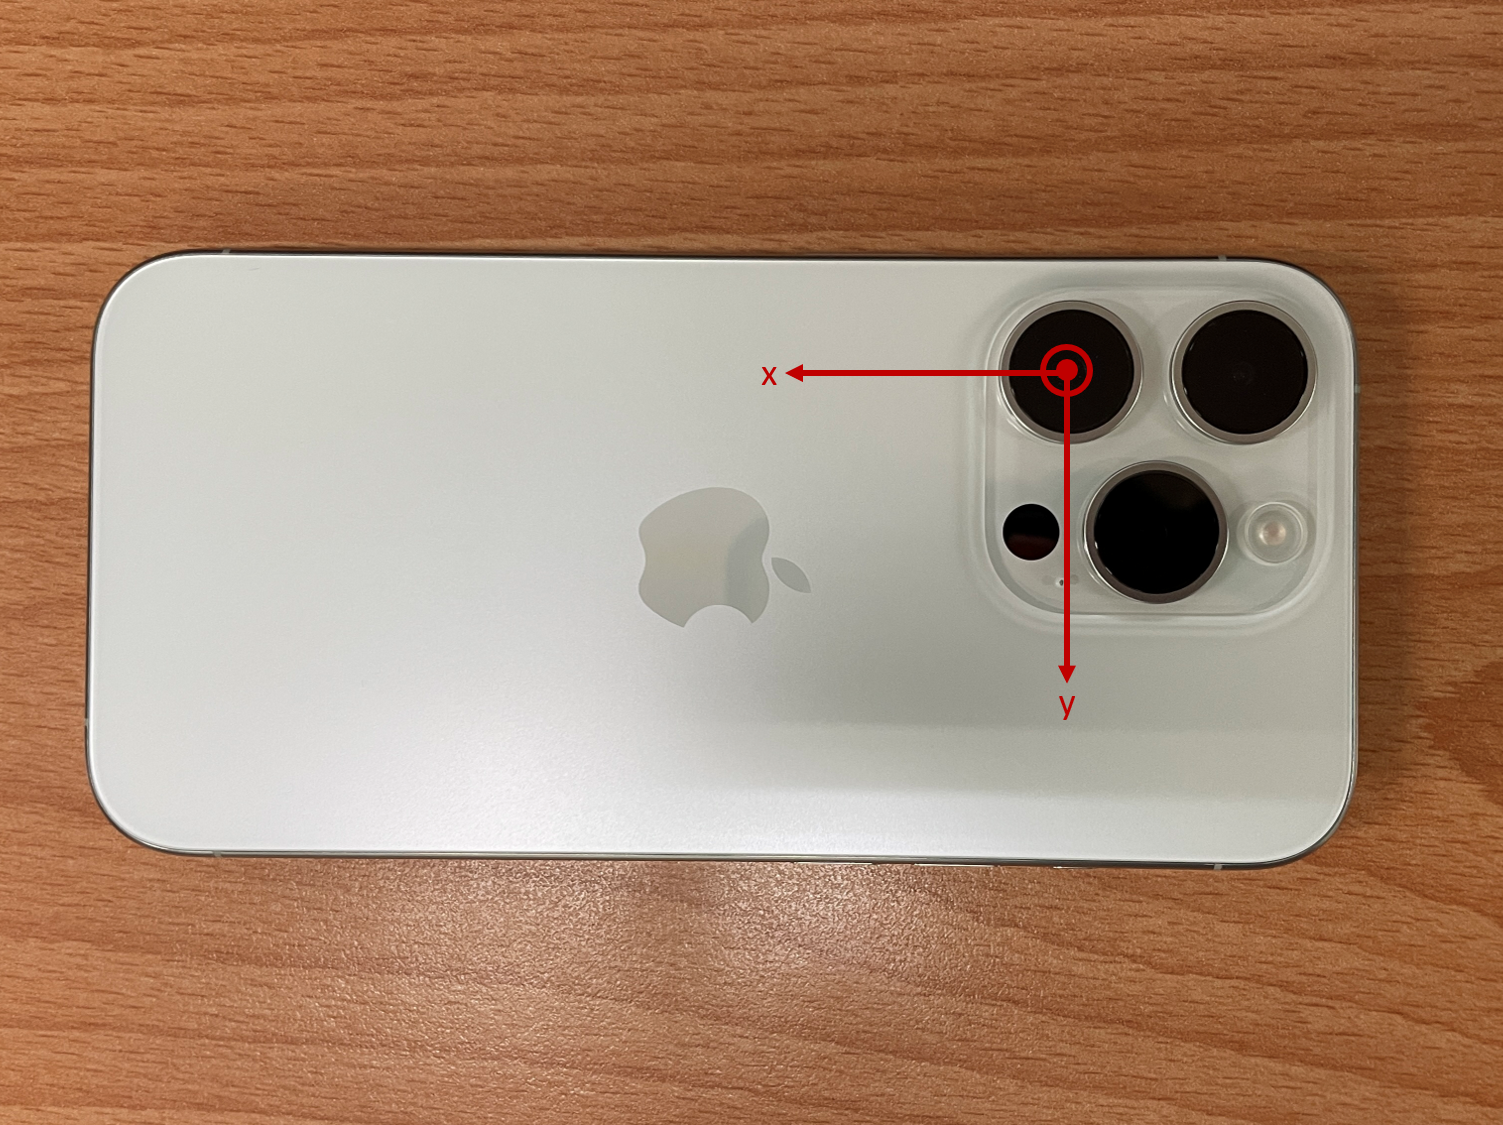
\includegraphics[width=.95\linewidth]{figure/ch3_fig_camframe.png}
      \caption*{(b) 相機座標系}
   \end{minipage}
   \begin{minipage}{.5\textwidth}
     \centering
     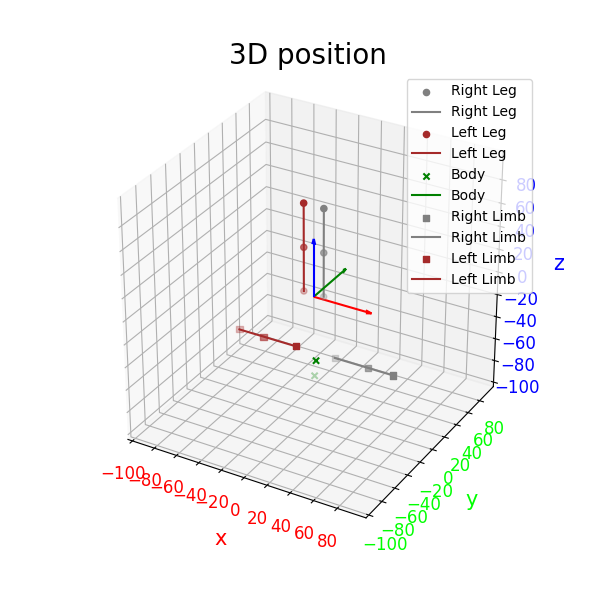
\includegraphics[width=.95\linewidth]{figure/ch3_fig_skeleton_frame.png}
     \caption*{(c) 人體模型座標系}
   \end{minipage}%
   \begin{minipage}{.5\textwidth}
     \centering
     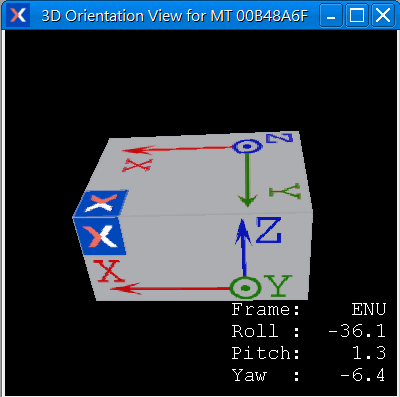
\includegraphics[width=.95\linewidth]{figure/ch3_fig_imu_frame.png}
     \caption*{(d) 感測器座標系}
   \end{minipage}
   \captionsetup{justification=centering}
   \caption[座標系定義]{座標系定義}
   \label{ch3_fig_frame}
\end{figure}

\clearpage

\subsubsection{各座標系間的關係}
% 各座標系間的關係介紹
在影像系統座標系定義與轉換的部分,本研究使用關係式~\ref{ch3_equ_image_rotation_matrix},
將在空間中的位置點由以全域座標系為表示方式轉換至以相機座標系為表示方式。

\begin{equation}
   R^{cam}_{g} = R^{cam}_{img}(R^{g}_{img})^{-1}
   \label{ch3_equ_image_rotation_matrix}
\end{equation}

其中,$R^{cam}_g$ 為將空間中的位置點由全域座標系轉換至相機座標系之旋轉矩陣,
即圖~\ref{ch3_fig_coordinate_trans} 中,從綠色座標系轉換至紫色座標系之旋轉矩陣,
通過將 $R^{cam}_g$ 乘以全域座標系中的人體模型朝向,將以全域座標系表示之朝向轉換為以相機座標系表示的人體模型朝向;
$(R^{g}_{img})^{-1}$ 為全域座標系轉換至圖像座標系之旋轉矩陣,
即圖~\ref{ch3_fig_coordinate_trans} 中,從綠色座標系轉換至粉色座標系之旋轉矩陣,
通過將 $R^{cam}_g$ 乘以全域座標系中的人體模型朝向,將以全域座標系表示之朝向轉換為以圖像座標系表示的人體模型朝向;
$R^{cam}_{img}$ 為圖像座標系轉換至相機座標系之旋轉矩陣,
即圖~\ref{ch3_fig_coordinate_trans} 中,從粉色座標系轉換至紫色座標系之旋轉矩陣,
通過將 $R^{cam}_{img}$ 乘以圖像座標系中的人體模型朝向,將以圖像座標系表示之朝向轉換為以相機座標系表示的人體模型朝向。

在 IMU 感測器系統座標系定義與轉換的部分,
本研究參考文獻~\cite{malleson2017real}所提出之關係式~\ref{ch3_equ_imu_rotation_matrix},並進行修正以更有助於理解,
將每一關節點由以人體模型座標系為表示方式轉換至以全域座標系為表示方式。

\begin{equation}
   R^g_b=R^g_iR^i_s(R^b_s)^{-1}
   \label{ch3_equ_imu_rotation_matrix}
\end{equation}

其中,$R^g_b$ 為將 IMU 所附著的人體模型朝向由人體模型座標系轉換至全域座標系之旋轉矩陣,
即圖~\ref{ch3_fig_coordinate_trans} 中,從黑色座標系轉換至綠色座標系之旋轉矩陣,
通過將 $R^g_b$ 乘以人體模型座標系中的人體模型朝向,將以人體模型座標系表示之朝向轉換為以全域座標系表示的人體模型朝向;
$(R^b_s)^{-1}$ 為人體模型座標系轉換至感測器座標系之旋轉矩陣,
即圖~\ref{ch3_fig_coordinate_trans} 中,從黑色座標系轉換至紅色座標系之旋轉矩陣,
通過將 $(R^b_s)^{-1}$ 乘以人體模型座標系中的人體模型朝向,將以人體模型座標系表示之人體模型朝向轉換為以感測器座標系表示的人體模型朝向;
$R^i_s$ 為感測器座標系轉換至 IMU local 座標系之旋轉矩陣,
即圖~\ref{ch3_fig_coordinate_trans} 中,從紅色座標系轉換至藍色座標系之旋轉矩陣,
通過將 $R^i_s$ 乘以感測器座標系中的人體模型朝向,將以感測器座標系表示之人體模型朝向轉換為以 IMU local 座標系表示的人體模型朝向;
$R^g_i$ 為 IMU local 座標系轉換至全域座標系之旋轉矩陣,
即圖~\ref{ch3_fig_coordinate_trans} 中,從藍色座標系轉換至綠色座標系之旋轉矩陣,
通過將 $R^g_i$ 乘以 IMU local 座標系中的人體模型朝向,將以 IMU local 座標系表示之人體模型朝向轉換為以全域座標系表示的人體模型朝向。
上述所提及之每一旋轉矩陣的量測與計算方式將於後續進行介紹。

\begin{figure}[!ht]
   \centering
   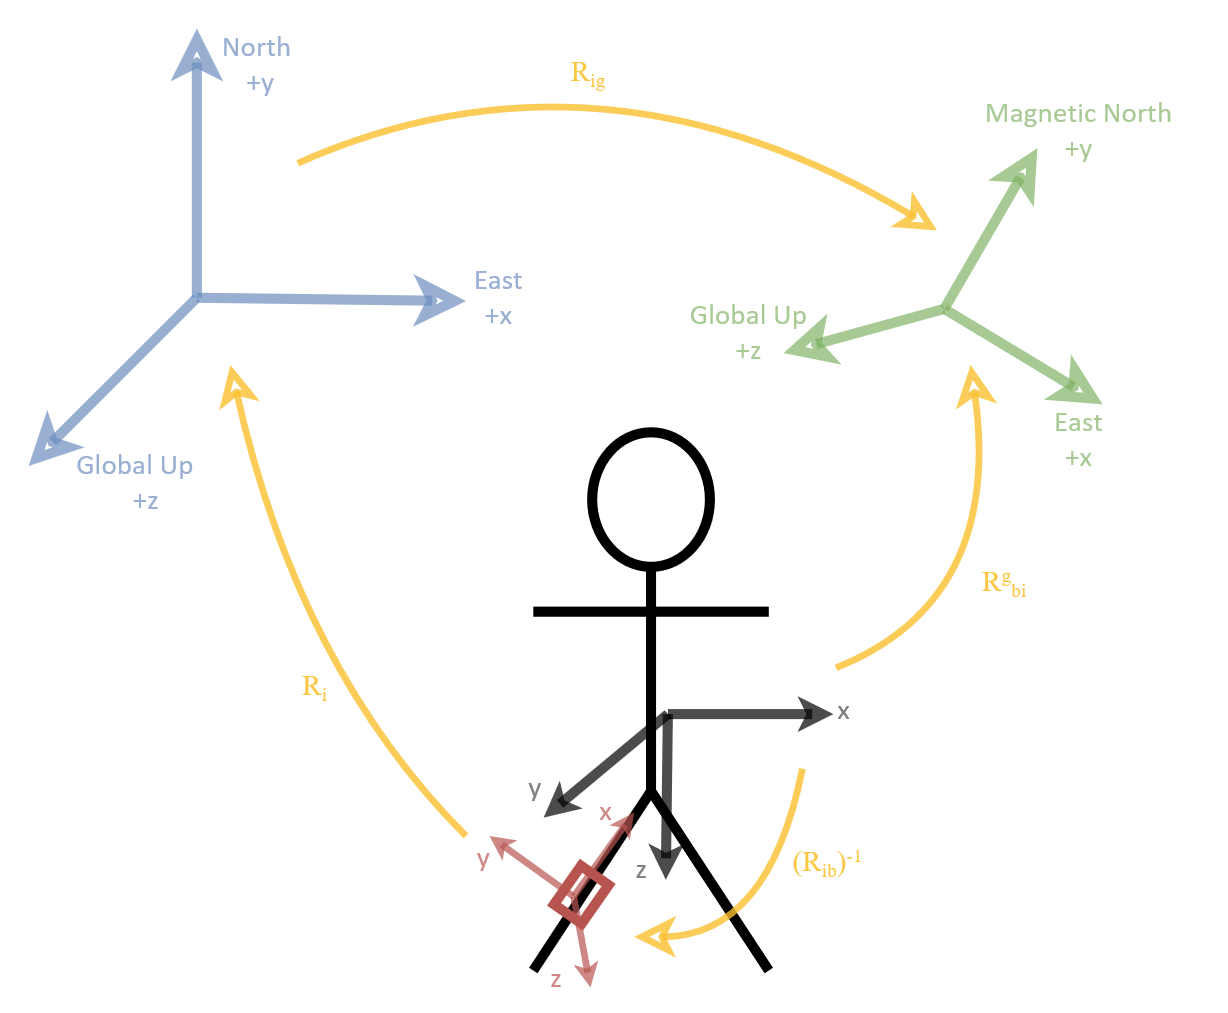
\includegraphics[width=\textwidth]{figure/ch3_fig_coordinate_trans.png}
    \caption[各座標系間的關係]{各座標系間的關係}
    \label{ch3_fig_coordinate_trans}
\end{figure}

\subsubsection{圖像座標 - 全域座標旋轉矩陣,$R^{g}_{img}$}
%圖像座標 - 全域座標旋轉矩陣
圖像座標 - 全域座標旋轉矩陣 ($R^{g}_{img}$) 為計算受試者手上棋盤格校正板與全域座標系間關係之旋轉矩陣,
其可將圖像座標系轉換至全域座標系,
將座標系統一轉換到全域座標系,以方便後續進行感測器融合計算。
圖像座標 - 全域座標旋轉矩陣計算方式如方程式~\ref{ch3_equ_img2g_rotation_matrix} ,
本研究將棋盤格校正板安裝上 IMU,並將棋盤格校正板的 x、y 座標方向與 IMU 的 x、y 對齊,
經過校正後,IMU 的朝向可直接視為棋盤格校正板的朝向,因此 $R^{i}_{img} = R^{i}_{s}$,
經由 IMU 量得的 IMU - IMU local 旋轉四元數即可視為棋盤格校正板 - IMU local 的旋轉四元數,
再將整體座標系對 y 軸旋轉 $90^{\circ}$ ,對 x 軸旋轉 $180^{\circ}$ ,即可得到圖像座標 - 全域座標旋轉矩陣。

\begin{equation}
   R^{g}_{img} = R_{x}(\theta_{x})R{y}(\theta_{y})R^{i}_{img} = R_{x}(\theta_{x})R{y}(\theta_{y})R^{i}_{s}
   \label{ch3_equ_img2g_rotation_matrix}
\end{equation}

\subsubsection{圖像座標 - 相機座標旋轉矩陣,$R^{cam}_{img}$}
% 圖像座標 - 相機座標旋轉矩陣
圖像座標 - 相機座標旋轉矩陣 ($R^{cam}_{img}$) 為計算受試者手上棋盤格校正板與相機間關係之旋轉矩陣,
其可將圖像座標系轉換至相機座標系,
本研究之計算方式為使用一 5x4,方格寬度為 50 (mm) 的棋盤格校正板,
並使用 Pose2Sim ~\cite{Pagnon_2022_JOSS}~\cite{Pagnon_2021_Robustness}~\cite{Pagnon_2022_Accuracy} 提供的校正工具進行外部參數及內部參數計算,
透過相機校正所得之外部參數即為棋盤格校正板與相機間的旋轉及平移關係。

\subsubsection{感測器座標 - 人體模型座標旋轉矩陣,$R^b_s$}
% IMU - 人體模型座標轉換矩陣計算介紹
% 解釋表示方法是以哪個座標系去看哪個座標系,然後解釋計算方法
使用 IMU 進行肢體朝向量測時,由於 IMU 黏貼於肢體上的方向及位置可能會和人體模型定義之方向及位置有所偏差,
因此需使用感測器座標 - 人體模型座標旋轉矩陣($R^b_s$),將位於感測器座標系的量測數值轉換為以人體模型座標系表示的人體模型朝向。
感測器座標 - 人體模型座標旋轉矩陣計算方式如方程式~\ref{ch3_equ_b2s_rotation_matrix},
假設受試者在最初始開始實驗時,設定一個與 IMU local 座標系對齊的人體模型座標系統,且受試者的姿勢為 T-pose,
因此此時 IMU 到其附著肢段的旋轉矩陣與 IMU 到 IMU local 的旋轉矩陣相同,即 $R^{b}_{s}(t_0) = R^{i}_{s}(t_0)$,
因此,在 $t_0$ 時刻量得的 IMU - IMU local 旋轉四元數即可視為感測器座標 - 人體模型座標旋轉四元數,
而由於在章節~\ref{ch3_skeleton_method} 中建立的人體模型座標與 IMU 附著於人體模型定義的座標系相差 $180^{\circ}$,
因此,再將整體座標系對 x 軸旋轉 $180^{\circ}$ ,即可得最終感測器座標 - 人體模型座標旋轉矩陣。 

\begin{equation}
   R^{b}_{s} = R_{x}(\theta_{x})R^{b}_{s}(t_0) = R_{x}(\theta_{x})R^{i}_{s}(t_0)
   \label{ch3_equ_b2s_rotation_matrix}
\end{equation}

% 此矩陣可經由 OpenSim~\cite{delp2007opensim}處理並進一步計算而得,其取得及計算方式如下。
% 首先,量測結束之 IMU 資料將透過 OpenSim 軟體進行處理,\sout{使用基礎人體模型模型...},計算每一 IMU 相對其對應人體模型之相對位置及角度,
% 處理結果可經由 OpenSim 軟體可視化,如圖~\ref{ch3_fig_imu_ori} 所示。
% 此項數據紀錄於 OpenSim 輸出之 .osim 檔案的 <BodySet> 元素中,<BodySet> 以人體模型為單位,
% 其中包含之 <components> 則記錄一附著於該人體模型上之 IMU 的相對位置及角度,
% <translation> 代表該 IMU 的原點相對於其附著之人體模型原點的平移,
% <orientation> 則代表該 IMU 的座標軸相對於其附著之人體模型坐標軸的旋轉。
% 因此若將 <translation> 數值更改為零,則可看到 IMU 原點與人體模型原點重合,如圖~\ref{ch3_fig_imu_tra},
% 而若將 <orientation> 數值更改為零,則可看到 IMU 坐標軸與人體模型坐標軸平行,如圖~\ref{ch3_fig_imu_rot}。
% 因此,從 .osim 檔案取得每一 IMU 相對於人體模型之相對位置及角度後,即可計算出感測器座標 - 人體模型座標四元數。
% \begin{figure}[!ht]
%    \centering
%    \begin{minipage}{.3\textwidth}
%      \centering
%      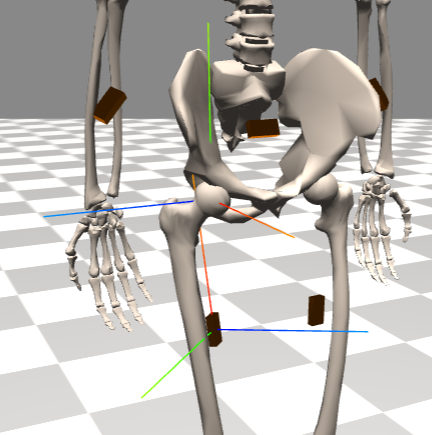
\includegraphics[width=.8\linewidth, height=.8\linewidth]{figure/ch3_fig_imu_ori.png}
%      \caption[OpenSim 計算結果]{OpenSim 計算結果}
%      \label{ch3_fig_imu_ori}
%    \end{minipage}%
%    \begin{minipage}{.3\textwidth}
%      \centering
%      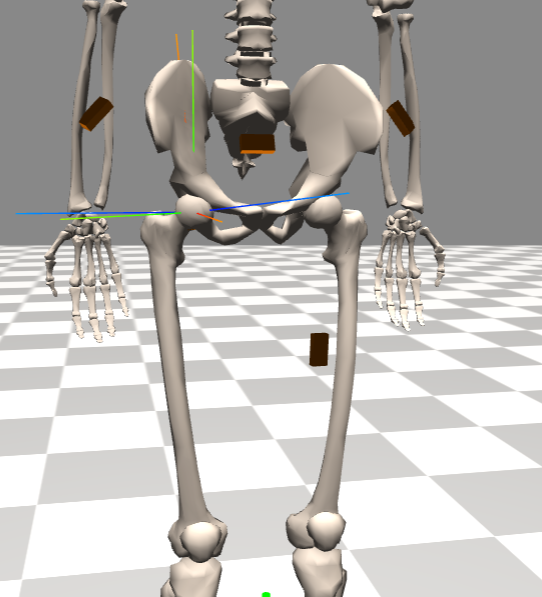
\includegraphics[width=.8\linewidth, height=.8\linewidth]{figure/ch3_fig_imu_tra.png}
%      \caption[IMU 平移為零]{IMU 平移為零}
%      \label{ch3_fig_imu_tra}
%    \end{minipage}%
%    \begin{minipage}{.3\textwidth}
%       \centering
%       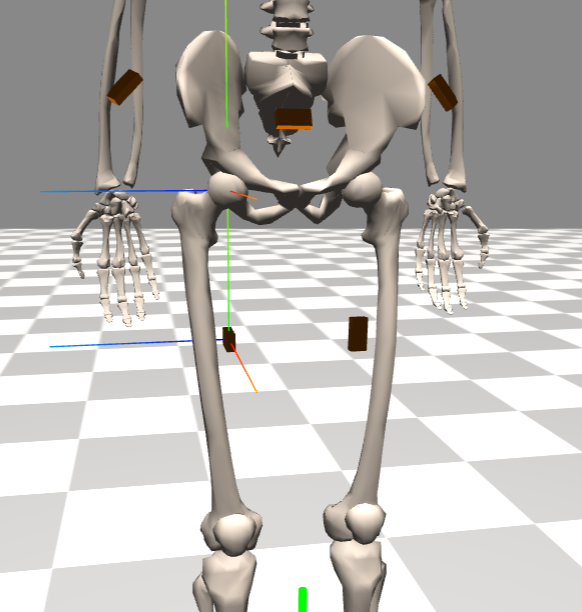
\includegraphics[width=.8\linewidth, height=.8\linewidth]{figure/ch3_fig_imu_rot.png}
%       \caption[IMU 旋轉為零]{IMU 旋轉為零}
%       \label{ch3_fig_imu_rot}
%     \end{minipage}
% \end{figure}

\subsubsection{感測器座標 - IMU local 旋轉矩陣,$R^i_s$}
經過上一步 $(R^b_s)^{-1}$ 的轉換,已將人體模型朝向轉換為以附著其上的 IMU 感測器座標系為表示方式,
接著,需要進一步將各自表示的感測器座標系轉換至統一以東北天 (East - North - Up, ENU) 為定義的 IMU local 座標系。
感測器座標 - IMU local 旋轉矩陣 ($R^i_s$) 為 IMU 的量測朝向,可直接經由 Xsens 系統所提供軟體 (MT manager) 輸出四元數取得。
在 MT manager 中讀入量測時所記錄的檔案,
% TODO:...模型為基礎
% 並於 file>export 中的輸出選項勾選 quaternion 後輸出,
每一輸出檔案中的 q0、q1、q2、q3 即為將朝向旋轉乘以 IMU local 座標系為表示方式的旋轉四元數,分別代表四元數的 w、x、y、z,
將四元數轉換為旋轉矩陣即可得感測器座標 - IMU local 旋轉矩陣。

\subsubsection{IMU local - 全域座標旋轉矩陣,$R^g_i$}
% IMU - 全域座標轉換矩陣計算介紹
% 解釋表示方法是以哪個座標系去看哪個座標系,然後解釋計算方法
經過上一步 $R^i_s$ 的轉換,已將人體模型朝向轉換為以統一的 IMU local 感測器座標系為表示方式,
接著,為方便後續與影像辨識而得的位置資訊進行融合,需要進一步將人體模型朝向轉換至位置資訊所在之座標系。
假設所有 IMU 間的 IMU local - 全域座標旋轉矩陣 $R^g_i$ 皆一致,此時兩者的座標相差 $-90^{\circ}$,因此需再對 Z 軸旋轉 $-90^{\circ}$,因此對 Z 軸旋轉 $-90^{\circ}$ 的旋轉矩陣即為 IMU local - 全域座標旋轉矩陣。
% 且與天頂及磁北極對齊,
% 再將整體座標系相對 x 軸旋轉 $-90^{\circ}$,即可得 IMU local - 全域座標旋轉矩陣。
% 包含兩個階段的旋轉,
% 第一階段先將於 IMU local 座標系的人體模型朝向轉換至以全域座標系表示,與天頂及磁北極校正,
% 第二階段將於全域座標系的人體模型朝向轉換至位置資訊所在之座標系,該座標系相對全域座標系的 x 軸旋轉 $-90^{\circ}$。
% 在第一階段中,IMU local - 全域座標的轉換與磁偏角 ($\delta$) 有關,
% 將 IMU local 座標系繞 z 軸旋轉 $\delta$ 即可轉換至全域座標系。
% 第二階段再將全域座標系繞 x 軸旋轉 $-90^{\circ}$,轉換至位置資訊所在之座標系。

% ------------------------- 3.4 ------------------------- %
\section{感測器融合方法}
% 感測器融合方法介紹
本研究使用學者 Zhe Zhang 等人提出的感測器融合方法進行影像與 IMU 資訊的融合~\cite{Zhang_2020_CVPR}。
此方法以學者 Bin Xiao ~\cite{Xiao_2018_ECCV} 等人提出的影像辨識方法 SimpleNet 作為基本框架,
並套入 Zhe Zhang 等人訓練的 $occlusion\_person\_8view.pth$ 模型進行影像辨識~\cite{zhang2020adafuse},
取得紀錄關節點於影像中位置的初步熱圖 (每一張熱圖僅記錄一個關節點的可能位置,因此同一時刻共會輸出 16 張關節點熱圖)。
由於初步熱圖可能存在辨識錯誤,因此會再使用 IMU 朝向資料進行同視角融合及跨視角融合。

\subsection{同視角融合}
假設有一關節點 $J_1$,其對應到影像熱圖 $H_1$ 中的點 $Y_P$,如圖~\ref{ch3_fig_joint_project} 所示,
且此關節點在空間中的位置必位於相機中心 $C_1$ 與影像熱圖中點 $Y_P$ 的延伸線上,
因此在直線上均勻取 $K$ 個樣本點 $P_k$, $k = 1, ..., K$,
利用這些樣本點及 IMU 的朝向資訊 $o$ 與三維人體模型肢段長度 $l$ 資訊,輸入式~\ref{ch3_equ_cal_qk} 中,推斷 $J_1$ 的子關節點 $J_2$ 應位於空間中的位置 $Q_k$, $k = 1, ..., K$ 之中,
將空間中的位置 $Q_k$ 投影至關節點 $J_2$ 的影像熱圖 $H_2$ 中,得 $Y^1_{Q_k}$, $k = 1, ..., K$。

\begin{equation}
   Q_k=P_k+o*l, \forall k=1,...,K
   \label{ch3_equ_cal_qk}
\end{equation}

理論上,與 $Y_P$ 相對應的 $Y_{Q_k}$ 的投影位置在熱圖 $H_2$ 上會有很高的數值,藉此提高 $J_1$ 在 $H_1$ 的位置是 $Y_P$ 的機率。但由於缺乏影像的深度資訊,無法得知真正與 $Y_P$ 對應的 $Y_{Q_k}$ 為何,因此 $Y_{Q_k}$ 會一併增加線上的所有網格點的機率,如圖~\ref{ch3_fig_fusion_result} (a),可發現圖中有一條明顯的線條,即為 $J_2$ 的可能位置。

% \begin{figure}[!ht]
%    \centering
%    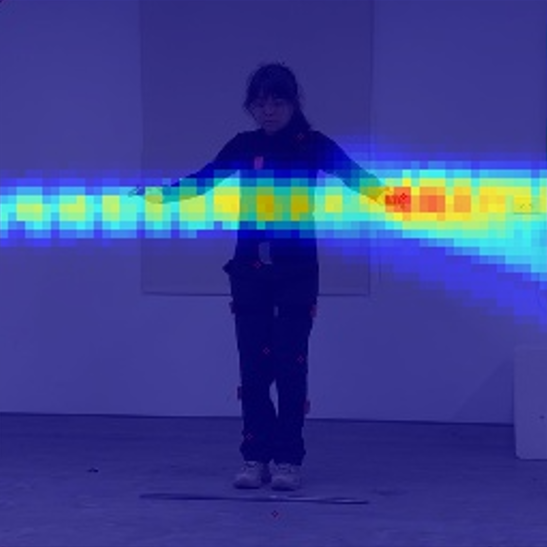
\includegraphics[width=8cm]{figure/ch3_fig_same_view.png}
%     \caption[同視角融合結果]{同視角融合結果}
%     \label{ch3_fig_same_view}
% \end{figure}

\subsection{跨視角融合}
從同視角融合可得到每一視角下被增加機率的格點,這條線上包含與 $Y_P$ 對應的格點及不與 $Y_P$ 對應的格點,也就是說與 $Y_P$ 不相關的格點的機率也被提高,但是,由於每一視角的線條中必存在一個正確的 $Y_{Q_k}$,因此,透過跨視角融合,將每一視角的熱圖與 $J_2$ 的初始熱圖 $H_2$ 進行疊加後取熱圖中的最大值即為 $Y_{Q_k^*}$,進而提高 $J_1$ 在 $H_1$ 的位置是 $Y_P$ 的機率。如圖~\ref{ch3_fig_fusion_result} (b),可發現圖中有兩條明顯的線條,其交點即為正確的關節點位置。

% \begin{figure}[!ht]
%    \centering
%    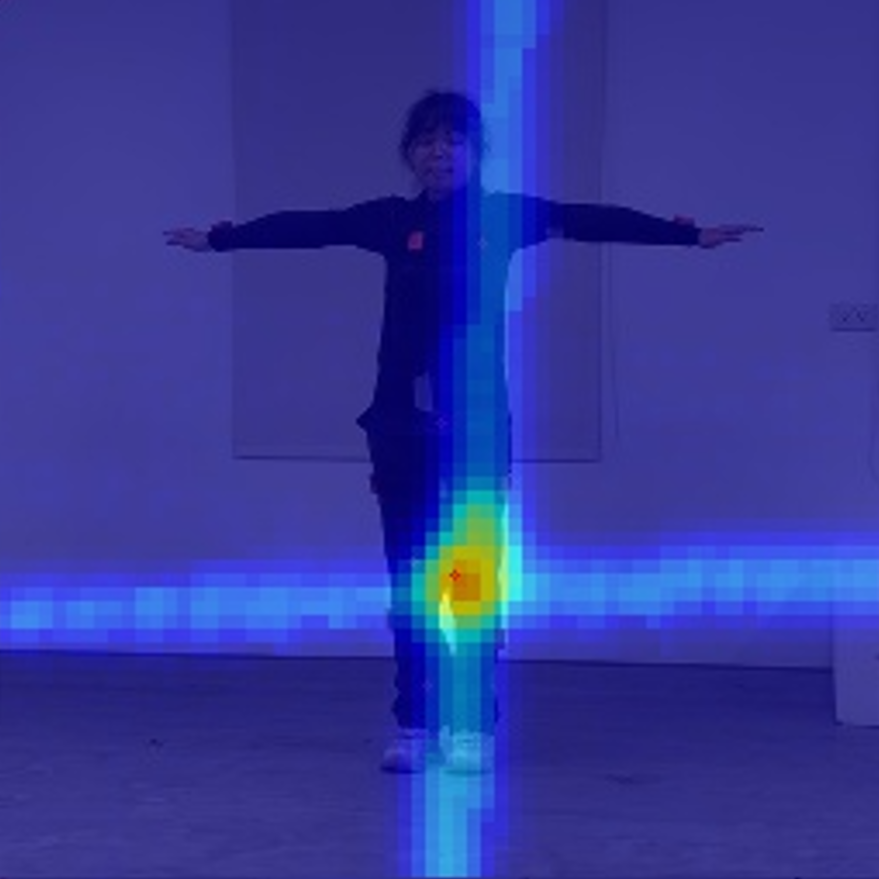
\includegraphics[width=8cm]{figure/ch3_fig_cross_view.png}
%     \caption[跨視角融合結果]{跨視角融合結果}
%     \label{ch3_fig_cross_view}
% \end{figure}

\begin{figure}[!ht]
   \centering
   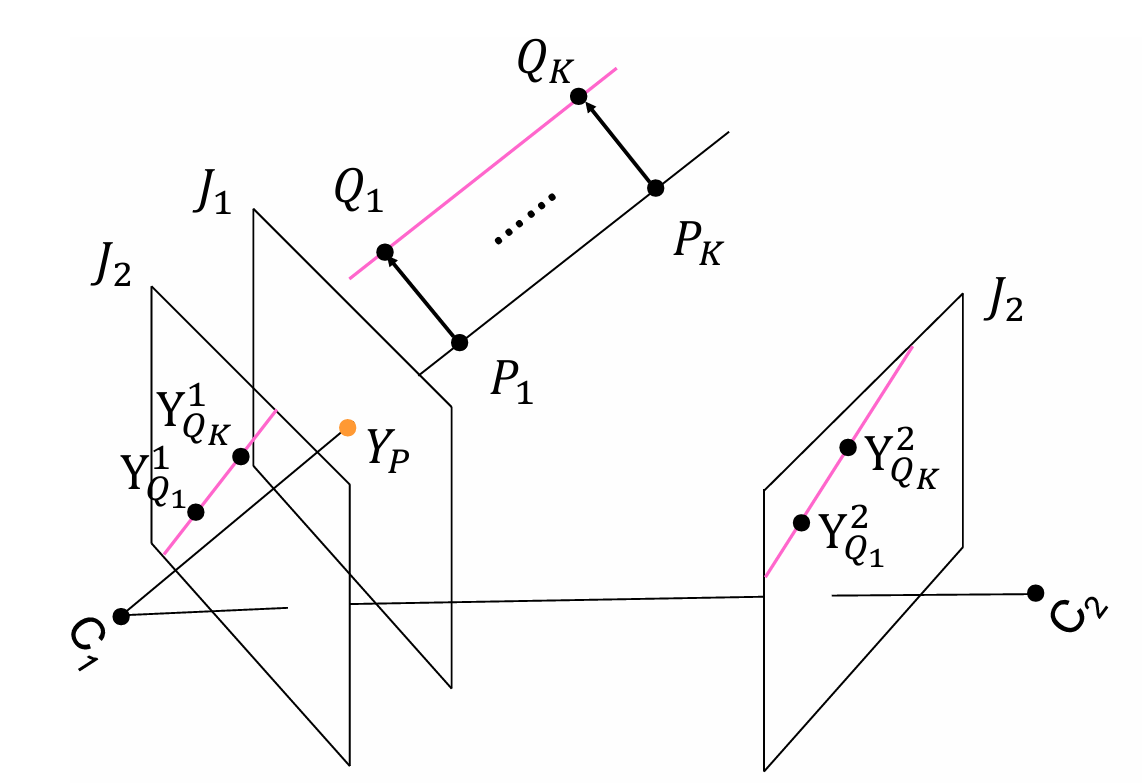
\includegraphics[width=10cm]{figure/ch3_fig_joint_project.png}
    \caption[影像與 IMU 同視角融合方法~\cite{Zhang_2020_CVPR}]{影像與 IMU 同視角融合方法~\cite{Zhang_2020_CVPR}}
    \label{ch3_fig_joint_project}
\end{figure}

\begin{figure}[!ht]
   \centering
   \begin{minipage}{.45\textwidth}
      \centering
      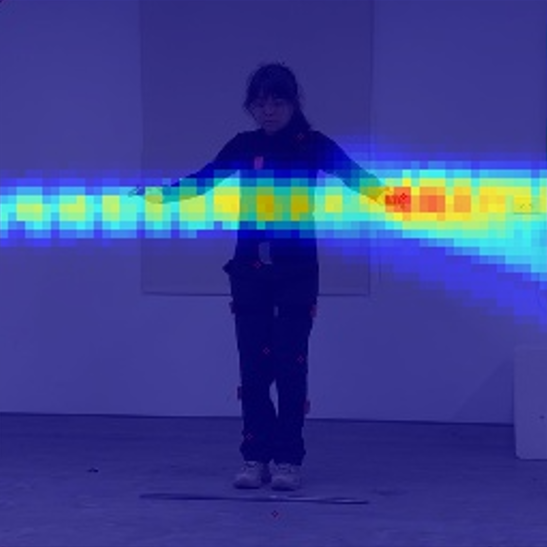
\includegraphics[width=.95\linewidth]{figure/ch3_fig_same_view.png}
      \caption*{(a) 同視角融合結果}
   \end{minipage}%
   \vspace{5mm}%
   \begin{minipage}{.45\textwidth}
      \centering
      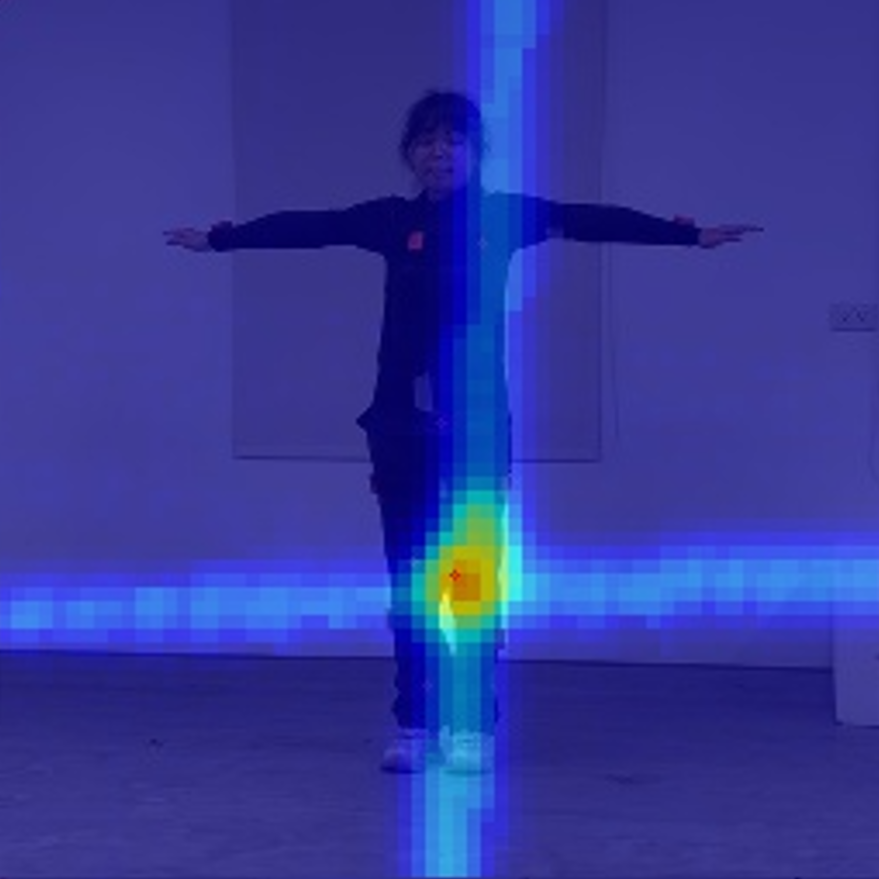
\includegraphics[width=.95\linewidth]{figure/ch3_fig_cross_view.png}
      \caption*{(b) 跨視角融合結果}
   \end{minipage}
   \captionsetup{justification=centering}
   \caption[感測器融合結果]{感測器融合結果}
   \label{ch3_fig_fusion_result}
\end{figure}

\clearpage

% ------------------------- 3.5 ------------------------- %
\section{人體姿態估計結果評估與驗證}
經過感測器融合後,將得到 16 個關鍵點的三維座標,分別為鼻子、頸部、肚子、左右肩膀、左右手肘、左右手腕、骨盆中點、左右骨盆、左右膝蓋、左右腳踝。多數學者將估計位置點直接與 Vicon 量測位置點進行比對,計算 MPJPE 數值,也有少數學者使用目視檢查的方式,決定位置跟蹤結果是否符合人體姿態~\cite{nakano2020evaluation},因此本研究將人體姿態估計結果驗證分為三個步驟,分別為檢查結果與人體是否相似、計算誤差及決定是否估計成功。

本研究將實驗結果每 20 幀進行一次取樣,等同於約 $\frac{1}{3}$ 秒取樣一次。每一樣本皆進行如圖~\ref{ch3_fig_est_flow} 的評估及驗證,首先以人工目視檢查重建結果是否符合人體姿態,符合則分別取肩膀、手肘、手腕、骨盆、膝蓋、腳踝共 12 個關節點計算肢段長度,並與受試者實際肢段長度相減取絕對值,再取平均,如式~\ref{ch3_equ_error},若平均差值小於 10 公分,則將該樣本點視為估計成功,同時計入估計成功次數,反之若平均差值大於 10 公分,則將該樣本視為估計失敗,不計入估計成功次數。最後將估計成功次數與總樣本數相除,如式~\ref{ch3_equ_success_rate},即為該實驗的成功率。

\begin{equation}
   error = \frac{\sum(\mid\text{估計肢段長度} - \text{實際肢段長度}\mid)}{8}
   \label{ch3_equ_error}
\end{equation}

\begin{equation}
   success\_rate = \frac{\text{成功次數}}{\text{樣本數}}
   \label{ch3_equ_success_rate}
\end{equation}

\begin{figure}[!ht]
   \centering
   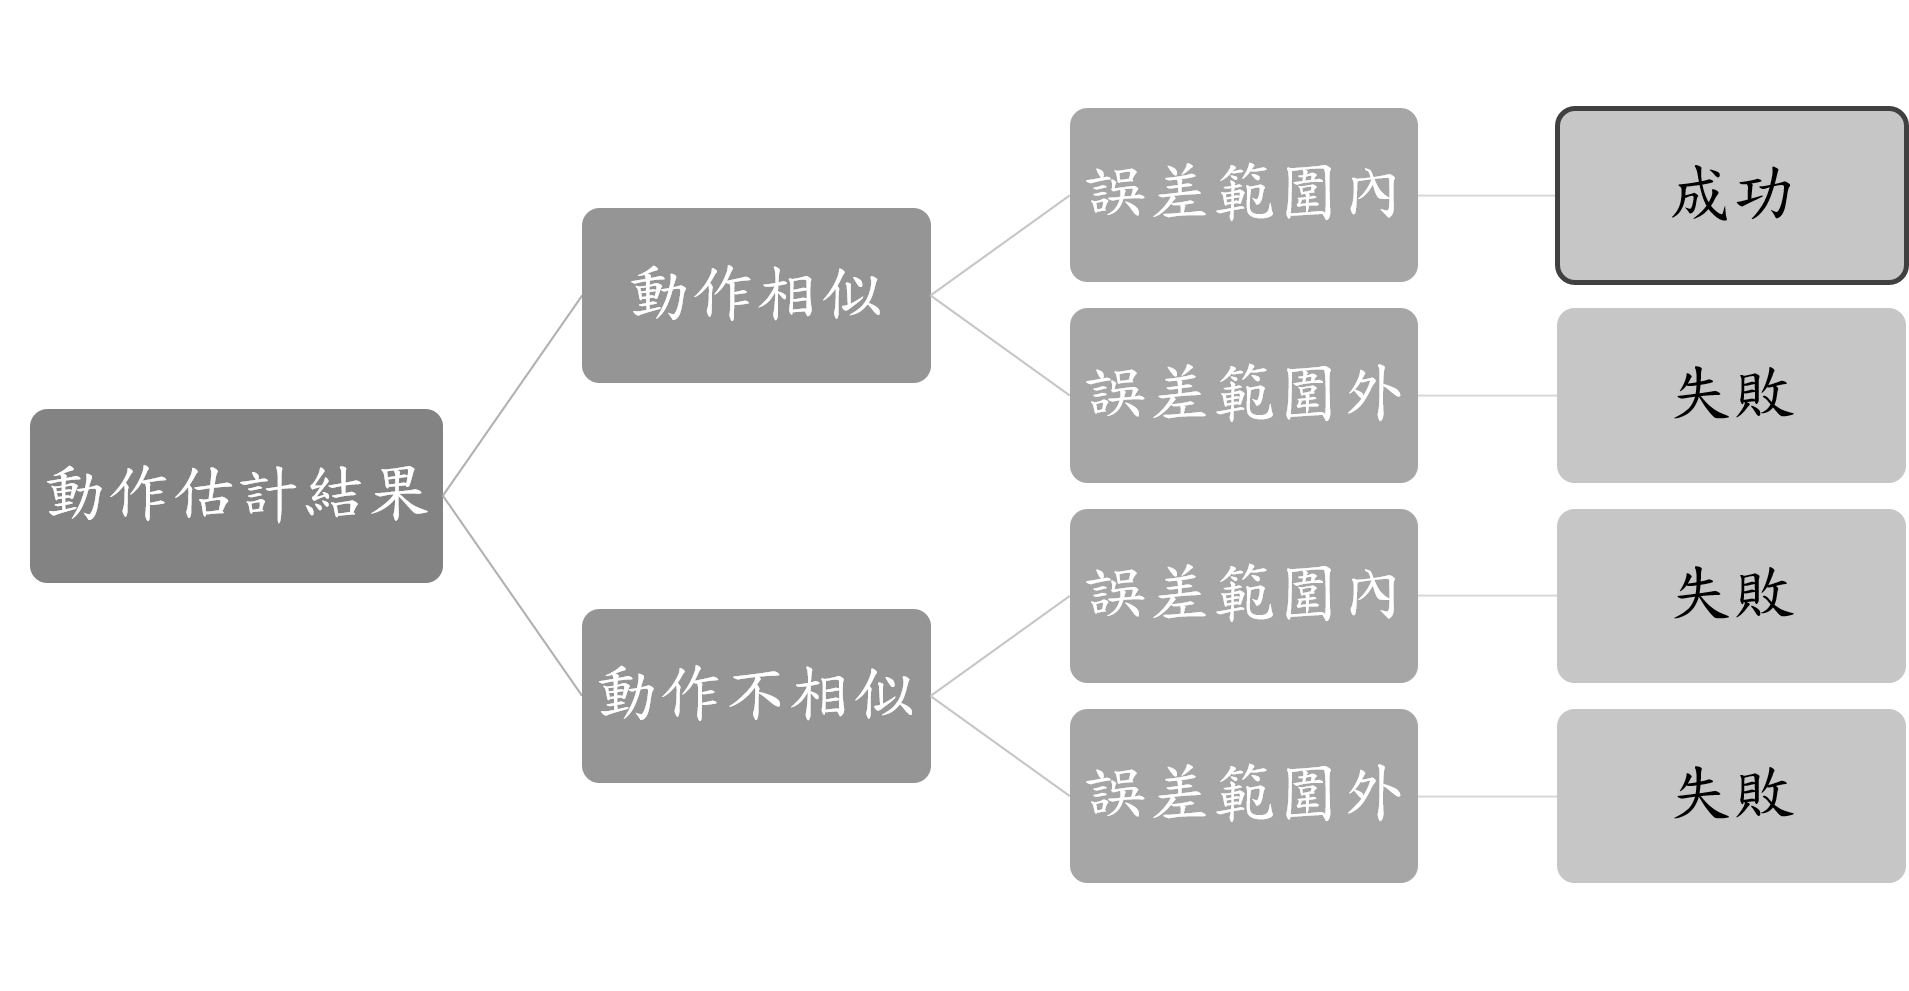
\includegraphics[width=11cm]{figure/ch3_fig_est_flow.png}
    \caption[評估重建結果流程]{評估重建結果流程}
    \label{ch3_fig_est_flow}
\end{figure}

\clearpage

% ------------------------- 3.6 ------------------------- %
\section{人體姿態估計結果可視化}
% 結果可視化介紹
% 分類成五個部分,分別用甚麼顏色表示
感測器融合方法共計算出 16 個關鍵點的三維座標,
分別為鼻子、頸部、肚子、左右肩膀、左右手肘、左右手腕、骨盆中點、左右骨盆、左右膝蓋、左右腳踝,
為方便觀察人體姿態,本研究使用 Matplotlib ~\cite{Hunter:2007} 繪製三維人體模型,
並將 16 個關鍵點分組至五個部位,分別以不同顏色表示,如圖~\ref{ch3_fig_posevis} 所示,
鼻子、頸部、肚子、骨盆中點分配至 body,以綠色表示,
右肩膀、右手肘、右手腕分配至 right arm,以藍色表示,
左肩膀、左手肘、左手腕分配至 left arm,以紫色表示,
右骨盆、右膝蓋、右腳踝分配至 right leg,以紅色表示,
左骨盆、左膝蓋、左腳踝分配至 left leg,以橘色表示。

\begin{figure}[!ht]
   \centering
   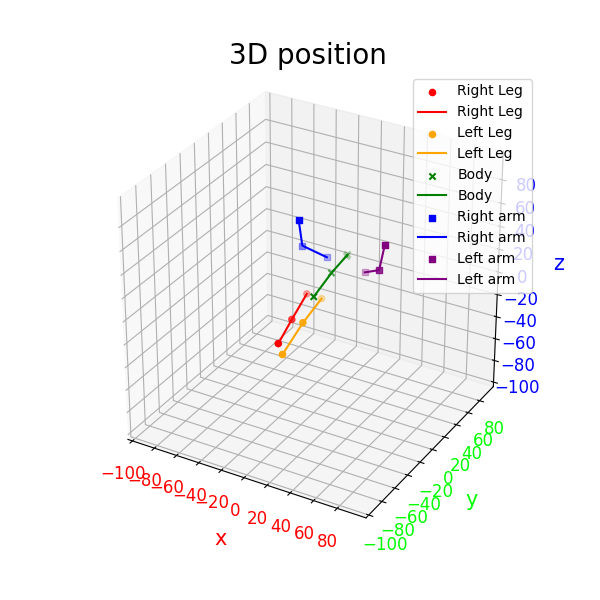
\includegraphics[width=11cm]{figure/ch3_fig_posevis.png}
    \caption[人體姿態可視化]{人體姿態可視化}
    \label{ch3_fig_posevis}
\end{figure}

\clearpage

% ------------------------- 3.6 ------------------------- %
\section{小結}
% 本章架構
本章節首先提出探討減少相機使用數量對於人體姿態估計精準度的影響的實驗方法與流程,並介紹實驗所需的硬體設備及軟體工具。接著,說明感測器融合前的資料前處理方法,包含相機校正、個人化三維人體模型建立方法、時間同步及空間校正。最後介紹感測器融合方法及人體姿態估計結果可視化方法。

% 應用
藉由上述方法,本研究將改善前人研究中部份資訊需透過 Vicon 系統進行補足的問題,同時藉由資料前處理方法,使受試者蒐集的量測資訊可輸入至感測器融合方法中,進行人體姿態估計,並透過人體姿態可視化方法,使研究者能夠直觀地觀察受試者的人體姿態,進而進行後續的研究分析。下個章節將依據本章的研究方法,完整介紹實驗設定,並針對實驗結果進行探討。
\clearpage